\documentclass[11pt,]{article}
\usepackage{lmodern}
\usepackage{amssymb,amsmath}
\usepackage{ifxetex,ifluatex}
\usepackage{fixltx2e} % provides \textsubscript
\ifnum 0\ifxetex 1\fi\ifluatex 1\fi=0 % if pdftex
  \usepackage[T1]{fontenc}
  \usepackage[utf8]{inputenc}
\else % if luatex or xelatex
  \ifxetex
    \usepackage{mathspec}
  \else
    \usepackage{fontspec}
  \fi
  \defaultfontfeatures{Ligatures=TeX,Scale=MatchLowercase}
\fi
% use upquote if available, for straight quotes in verbatim environments
\IfFileExists{upquote.sty}{\usepackage{upquote}}{}
% use microtype if available
\IfFileExists{microtype.sty}{%
\usepackage{microtype}
\UseMicrotypeSet[protrusion]{basicmath} % disable protrusion for tt fonts
}{}
\usepackage[margin=1.0in]{geometry}
\usepackage{hyperref}
\hypersetup{unicode=true,
            pdftitle={The fecal microbiome as a tool for monitoring and predicting response outcomes in Ustekinumab-treated, anti-TNF-alpha refractory Crohn's Disease patients.},
            pdfborder={0 0 0},
            breaklinks=true}
\urlstyle{same}  % don't use monospace font for urls
\usepackage{graphicx,grffile}
\makeatletter
\def\maxwidth{\ifdim\Gin@nat@width>\linewidth\linewidth\else\Gin@nat@width\fi}
\def\maxheight{\ifdim\Gin@nat@height>\textheight\textheight\else\Gin@nat@height\fi}
\makeatother
% Scale images if necessary, so that they will not overflow the page
% margins by default, and it is still possible to overwrite the defaults
% using explicit options in \includegraphics[width, height, ...]{}
\setkeys{Gin}{width=\maxwidth,height=\maxheight,keepaspectratio}
\IfFileExists{parskip.sty}{%
\usepackage{parskip}
}{% else
\setlength{\parindent}{0pt}
\setlength{\parskip}{6pt plus 2pt minus 1pt}
}
\setlength{\emergencystretch}{3em}  % prevent overfull lines
\providecommand{\tightlist}{%
  \setlength{\itemsep}{0pt}\setlength{\parskip}{0pt}}
\setcounter{secnumdepth}{0}
% Redefines (sub)paragraphs to behave more like sections
\ifx\paragraph\undefined\else
\let\oldparagraph\paragraph
\renewcommand{\paragraph}[1]{\oldparagraph{#1}\mbox{}}
\fi
\ifx\subparagraph\undefined\else
\let\oldsubparagraph\subparagraph
\renewcommand{\subparagraph}[1]{\oldsubparagraph{#1}\mbox{}}
\fi

%%% Use protect on footnotes to avoid problems with footnotes in titles
\let\rmarkdownfootnote\footnote%
\def\footnote{\protect\rmarkdownfootnote}

%%% Change title format to be more compact
\usepackage{titling}

% Create subtitle command for use in maketitle
\newcommand{\subtitle}[1]{
  \posttitle{
    \begin{center}\large#1\end{center}
    }
}

\setlength{\droptitle}{-2em}
  \title{The fecal microbiome as a tool for monitoring and predicting response
outcomes in Ustekinumab-treated, anti-TNF-alpha refractory Crohn's
Disease patients.}
  \pretitle{\vspace{\droptitle}\centering\huge}
  \posttitle{\par}
  \author{}
  \preauthor{}\postauthor{}
  \date{}
  \predate{}\postdate{}

\usepackage{setspace}
\doublespacing
\usepackage{lineno}
\linenumbers
\renewcommand{\familydefault}{\sfdefault}
\usepackage{graphicx}

\begin{document}
\maketitle

\begin{verbatim}
##                   Clinical.Variable     Summary
## 1                              CDAI  rho = -0.2
## 2  Loose Stool Frequency (per week)  rho = -0.2
## 3   C-Reactive Protein (mg/L serum)  rho = 0.06
## 4         Fecal Calprotectin (µg/g)  rho = 0.08
## 5          Fecal Lactoferrin (µg/g)   rho = 0.1
## 6                               BMI  rho = 0.07
## 7                       Weight (kg)  rho = 0.07
## 8                       Age (years) rho = -0.05
## 9                         Sex (F/M)           -
## 10         Corticosteroid Use (Y/N)           -
## 11         Disease Duration (years)  rho = -0.2
## 12               Tissue Involvement           -
##    Species.Richness..Alpha.diversity. Community.Structure..beta.diversity.
## 1                               0.014                                0.324
## 2                               0.003                                0.024
## 3                               0.394                                0.033
## 4                               0.254                                0.006
## 5                                0.07                                0.004
## 6                               0.299                                0.277
## 7                               0.299                                0.112
## 8                               0.472                                0.033
## 9                               0.539                                0.277
## 10                              0.001                                 0.01
## 11                              0.001                                0.004
## 12                               0.19                                0.004
\end{verbatim}

\begin{verbatim}
## [1] 0.014
## Levels: 0.001 0.003 0.014 0.07 0.19 0.254 0.299 0.394 0.472 0.539
\end{verbatim}

\vspace{35mm}

Running title: Microbiome of Ustekinumab-treated Crohn's Disease
patients.

\vspace{35mm} Matthew K. Doherty\({^2}\), Tao Ding\({^2}\)\({^\alpha}\),
Charlie Koumpouras\({^2}\), Shannon Telesco\({^1}\), Calixte
Monast\({^1}\), and Patrick D. Schloss\({^2}\)\({^\dagger}\)

\(\dagger\) To whom correspondence should be addressed:
\href{mailto:pschloss@umich.edu}{\nolinkurl{pschloss@umich.edu}}

1. Janssen Pharmaceutical Companies of Johnson \({\&}\) Johnson, Spring
House, PA, USA

2. Department of Microbiology and Immunology, University of Michigan,
Ann Arbor, MI, USA

\({\alpha}\) Currently at Department of Biology, New York University,
New York, NY, USA.

\newpage

\subsection{Abstract}\label{abstract}

\emph{Abstract:} Crohn's disease (CD) is a global health issue
characterized by patches of ulceration and inflammation along the
gastrointestinal tract, as well as reduced gut microbial diversity. We
investigated the association between the fecal microbiome and clinical
phenotypes of subjects with moderate to severe CD that were refractory
to anti-TNFa and treated with Ustekinumab (UST). We hypothesized that
the fecal microbiome at baseline was predictive of disease severity and
therapeutic response and that the fecal microbiota would change as a
result of therapy. Stool samples from 500 patients taking part in a
double-blinded, placebo-controlled, Phase 2b clinical trial were
obtained over the course of 22 weeks. The V4 region of the 16S rRNA gene
was amplified and sequenced to determine the structure of the fecal
bacterial communities.

Fecal microbial diversity at baseline was significantly correlated with
markers for disease severity, such as Crohn's Disease Activity Index
(CDAI), stool frequency, and disease duration. Additionally, stool
frequency, CRP, fecal lactoferrin, fecal calprotectin, corticosteroid
use, disease duration, and tissue involvement had a significant effect
on the \({\beta}\)-diversity of the microbiome. Baseline fecal
microbiome community structures and \({\alpha}\)-diversity were
significantly different based on the outcome of UST treatment.
\emph{Faecalibacterium}, among other taxa, was significantly more
abundant in responders/remitters. Additionally, the microbiome of
clinical responders changed over time, in contrast to nonresponsive
subjects. Using Random Forest models, the differences in the baseline
microbiome and clinical metadata could effectively predict therapeutic
outcome, especially for remission.

\emph{Importance:} The ability to predict and monitor response to
treatment using the microbiome will provide another clinical tool in
treating CD patients. Additionally, the observed baseline differences in
fecal microbiota and changes due to therapeutic response will allow
further investigation into the microbes and/or the metabolic functions
important in CD pathogenesis as well as establishing and maintaining CD
remission. Finally, beneficial microbes associated with response to
treatment could be developed therapeutics to increase the likelihood of
response while undergoing treatment.

\textbf{Keywords: Crohn's Disease, fecal microbiome, biologics,
prediction}

\newpage

\subsubsection{Introduction}\label{introduction}

Crohn's disease (CD), an incurable inflammatory bowel disease (IBD), is
a global health issue causing large economic and healthcare utilization
impacts on society (1--3). CD is characterized by patches of ulceration
and inflammation along the entire gastrointestinal tract, though mostly
the ileum and colon. Currently, individuals with CD are treated based on
disease location and risk of complications using escalating
immunosuppressive treatment, and/or surgery, with the goal of achieving
and sustaining remission (4, 5). Faster induction of remission following
diagnosis reduces the risk of irreversible intestinal damage and
disability (5--7). Ideally, clinicians would be able to determine
personalized treatment options for CD patients at diagnosis that would
result in faster achievement of remission {[}cites{]}. Therefore, recent
research has been focused on identifying noninvasive, prognostic
biomarkers to monitor CD severity and predict therapuetic response
{[}cites{]}.

The precise etiology of CD remains unknown, but host genetics,
environmental exposure, and the gut microbiome appear to be involved (1,
8). Individuals with CD have reduced microbial diversity in their guts,
compared to healthy individuals, with a lower relative abundance of
\emph{Firmicutes} and an increased relative abundance of
\emph{Enterobacteraciae} and \emph{Bacteroides}, at the phylum level
(9--13). Additionally, genome-wide association studies of individuals
with CD identified several susceptibility loci, including loci involved
in the IL-23 signialing pathway, which could impact the gut microbiome
structure and function (4, 9). If the fecal microbiome can be used to
monitor disease severity and predict response to specific treatment
modalities, then clinicians could use it as a noninvasive tool for
prescribing therapies that result in faster remission.

The microbiome has been correlated with a variety of diseases and has
shown promise as a predictive tool for disease outcome for
gingivitis(14), cardiovascular disease(15), \emph{Clostridium difficile}
infection (16--18), and colorectal cancer (19, 20). In relation to IBD,
previous studies have shown that the gut microbiome correlates with
disease severity in new-onset, pediatric CD patients (13, 21).
Additionally, recent studies have shown promise for the microbiome as it
relates to IBD and therapeutic response (22). It remains to be
determined, however, whether the fecal microbiome can predict and
monitor response to therapy in CD (9).

The FDA recently approved Ustekinumab (UST), a monoclonal antibody
directed against the shared p40 subunit of IL-12 and IL-23, for the
treatment of CD (5, 23--25). Given the potential impact of IL-23 on the
microbiome {[}cites{]}, we hypothesized that UST treatment may alter the
fecal microbiome and that response to UST could be predicted or
influenced by differences in patients' gut microbiota. We analyzed the
fecal microbiomes of individuals who participated in a double-blinded,
placebo-controlled Phase II clinical trial of UST in treating CD (23).
Using 16S rRNA gene sequence data from these patients' stool samples, we
determined associations between clinical metadata, disease severity, and
the fecal microbiome. We also tested whether the microbiome changed in
subjects with UST and if clinical responders had a microbiome that is
distinct from non-responders. Our study demonstrates that the fecal
microbiome is associated with baseline clinical metadata and that these
associations are useful in predicting and monitoring treatment outcome.

\subsection{Results}\label{results}

\textbf{Characteristics of the study population and their microbiomes
based on clinical variables}

We characterized the fecal microbiota in a subset of TNF-\({\alpha}\)
refractory CD patients, with moderate to severe CD, who took part in the
double-blinded, CERTIFI clinical trial (23). Demographic and baseline
disease characteristics of this subset are summarized in Table 1.
Patients were randomly assigned to a treatment group in the induction
phase of the study and at week 8 patients were re-randomized into
maintenance therapy groups based on their induction response (Figure
1A). Subjects provided stool samples at screening (week 0), week 4, week
6, and week 22 post induction for analysis using 16S rRNA gene
sequencing (Figure 1B).

Following sequence curation using the mothur software package (26), we
obtained a median of 13,732 sequences per sample (IQR = 7,863-21,978).
Parallel sequencing of a mock community had an error rate of 0.017\%. To
limit effects of uneven sampling, we rarefied the dataset to 3,000
sequences per sample. Samples from subjects that completed the clinical
trial and had complete clinical metadata were included in our analysis.
Of these samples, 306 were provided prior to treatment as well as 258
provided at week 4, 289 at week 6, and 205 at week 22 post-treatment,
for a total of 1058 samples.

We hypothesized that there were associations between the microbiome and
clinical variables at baseline related to disease severity in this
unique cohort. To test this hypothesis, we compared the week 0
microbiome with clinical data at week 0 (Supplemental Table 1). We
compared \({\alpha}\)-diveristy at baseline to clinical variables using
the inverse Simpson index with the Spearman correlation, wilcoxon, or
kurskal-wallis tests to compare groups. We compared
\({\beta}\)-diversity with a PERMANOVA using the adonis function in the
vegan R package. Following multiple comparison correction, we observed
small, but significant correlations for lower \({\alpha}\)-diversity
correlating with higher CDAI (rho = -0.161, p = 0.014), higher frequency
of loose stools per week (rho = -0.193, p = 0.003), and longer disease
duration (rho = -0.225, p = 0.001), with lower diversity corresponding
to longer disease. Corticosteroid use was associated with higher
\({\alpha}\)-diversity (p = 0.001). No significant association was
observed between \({\alpha}\)-diversity and CRP, fecal calprotectin, or
fecal lactoferrin. However, the \({\beta}\)-diversity was significantly
different based on CRP (p = 0.033), fecal calprotectin (p = ), and fecal
lactoferrin (p = ). The \({\beta}\)-diversity was also significantly
different based on weekly loose stool frequency (p= ), age (p = ), the
tissue affected (p = 0.004), corticosteroid use \({\beta}\)-diversity (p
=0.01) and disease duration (p = 0.004). No significant differences in
the microbiome were observed for BMI, weight, or sex.

\textbf{The microbiome by treatment and response over time}

Having established characteristics of the microbiome in our subjects at
baseline, we hypothesized that the microbiome could change as a result
of treatment. The effects of biologic treatment of IBD on the microbiome
are not yet well described, but are hypothesized to be indirect as these
drugs act on host factors that could influence the microbiome and not
microbes directly. We tested whether treatment with UST affects the
microbiome using subjects who provided samples at weeks 0, 4, and 6.
This allowed for us to analyze 156 treated subjects and 48 placebo
subjects with a sample at each time point. Using the adonis function in
the vegan R package (27), we performed a PERMANOVA stratified on each
subject, as a proxy for a repeated measures ANOVA, to determine if the
\({\beta}\)-diversity of microbiome changed over time. We included
induction treatment group, response at each clinical endpoint, and time
as parameters.

No significant difference was seen in community structure or
\({\alpha}\)-diversity based on sample date when looking at all
treatment groups and week 6 response status, but there was a significant
interaction between week 22 response and sample date (p = 0.001). There
was also a significant interaction and between week 22 responses,
induction group, and sample date (p = 0.044). This led us to further
examining the microbial community structures in week 22 responders and
non-responders over time by induction treatment. No significant
difference was observed in Week 22 non-responders over time, regardless
of treatment. In week 22 responders, we saw a significant change in
community structure over time in both placebo (p = 0.034) and UST
induction groups (p = 0.018).

Since we observed significant changes in the community structure of week
22 responders, we also hypothesized that treatment may also affect
\({\alpha}\)-diversity. We tested this by performing a Freidman test
comparing \({\alpha}\)-diversity at each sample date within each
induction treatment group based on their week 22 response status. As
seen in Figure 4, we saw no significant difference in
\({\alpha}\)-diversity over time in subjects who did not respond at week
22, regardless of induction treatment. However, in UST treated-week 22
responders \({\alpha}\)-diversity increased significantly from week 0 to
week 4 (p = 0.0022) and remained higher than baseline at week 6. This
change was not observed in subjects induced with placebo who responded
at week 22, unlike the community structure analysis. We hypothesize that
this reflects decreased inflammation in the subjects who responded to
treatment.

\textbf{The microbiome following treatment can distinguish between
treatment outcomes}

Having observed that the microbiome changes in subjects who responded to
treatment, we hypothesized that we could use the fecal microbiome to
distinguish between subjects who responsded to treatment from those who
did not respond. A paper recently published by Tedjo et al. demonstrated
a link between the microbiome and disease severity, where specific
microbes were associated with remission compared to active CD (28). We
hypothesized that the microbiome could be used to monitor response to
therapy in a similar manner. We used AUC-RF in order to determine if the
fecal microbiome at Week 6 could be used to determine if a study
participant responded to therapy or was in remission at Week 6. As seen
in Figure 5, using the microbiome alone we achieved an AUC of 0.708 for
response with a sensitivity of 0.769 and a specificity of 0.606. For
remission we had an AUC of 0.866 with a sensitivity of 0.833 and
specificity of 0.832. We were better able to distinguish remitters from
non-remitters than responders from non-responders. We hypothesize that
this is due to the relative nature of the response criteria compared to
the threshold used to determine remission status.

\textbf{Prediction of response based on the microbiome at screening}

Having demonstrated that the microbiome following treatement could
distinguish between outcomes, we hypothesized that the fecal microbiome
could predict response to therapy. To test this hypothesis, we used the
AUCRF package in R to develop a random forest classification model to
classify responders from non-responders, as well as remitters from
non-remitters, based on the relative abundance of fecal microbiome
community members, clinical metadata, and the combination of microbiome
and clinical data (20, 29). We ran these models for response and
remission at Week 6 and 22 of the study. The optimal models for response
and remission at the primary endpoint (Week 6) are shown in \emph{Figure
6A and C}. Using only clinical metadata, we achieved an AUC of 0.693, a
specificity of 0.76, and a sensitivity of 0.598. Using only microbiome
data, the model predicted response with an AUC of 0.737 with a
specificity of 0.807 and a sensitivity of 0.585. When combining clinical
metadata with the microbiome, the model predicted response with an AUC
of 0.745, a specificity of 0.727, and a sensitivity of 0.744. With
respect to Week 6 remission, using solely clinical metadata we achieved
AUC of 0.616 with a specificity of 0.801 and a sensitivity of 0.452.
Using only fecal microbiome data we achieved an AUC of 0.838 with a
specificity of 0.766 and a sensitivity of 0.806. When combining clinical
metadata with the microbiome, we achieved an AUC of 0.844 with a
specificity of 0.831 and a sensitivity of 0.774. Across all weeks and
responses, prediction with clinical metadata alone did not perform as
well as models using the fecal microbiome at screening. Also, combining
microbiome data with clinical metadata did not consistently improve
prediction compared to microbiome data alone. Additionally we found
several OTUs occurred frequently across models including
\emph{Faecalibacterium}, among other taxa that were more abundant in
responders/remitters (Figure 6B and D).

\textbf{Comparison of clinical responders and non-responders}

Given the observed differences in the fecal microbiome at baseline and
week 6 in responders/remitters compared to non-responders/non-remitters,
We hypothesized that there are associations between the microbiome at
baseline and treatment outcome. To test this, we compared the week 0
microbiomes of subjects based on treatment group and outcome status at
week 6 and week 22. Outcome status was broken into 2 catagories;
response and remission. Response is a relative value defined as a
decrease in a subject's initial CDAI of 30\% or more, while remission is
defined as a CDAI below the threshold of 150. For week 22 analysis,
subjects who changed treatment for maintainence therapy were not
included in our analysis. This resulted in 120 subjects induced and
maintained with UST and 25 subjects induced and maintained with placebo
included in our week 22 analysis. Week 6 analysis compared to the full
306 subjects with screening samples.

With respect to \({\alpha}\)-diversity, subjects induced with UST and in
remission at week 6 were significantly different from non-remitters
treated with UST, having higher diversity based on inverse Simpson
(respective median values = 11.6 (IQR = 4.66-13.9), 6.95 (IQR =
4.4-11.8), p = 0.020). No other treatment or response groups were
significantly different. Beta-diversity was significantly different for
each outcome status (response/remission) and treatment group at each
clinical endpoint (week 6 response p = 0.012, week 6 remission p =
0.017, week 22 response p = 0.012, week 22 remission p = 0.012), as seen
in Table 2. No phyla were significantly different by treatment and
response, however \emph{Fusobacteria} was less frequently observed in
week 6 remitters than non-remitters treated with UST (median relative
abundance = 0 (IQR = - ) and 0.0333 (IQR = - ), respectively).

As seen in Figure 3, two taxa were significantly more abundant in
UST-induced, week 6 remitters compared to non-remitters;
\emph{Bacteroides} (OTU0019) (p = 0.022) and \emph{Faecalibacterium}
(OTU0007) (p = 0.0026).

No individual taxa were significantly different among UST induced
subjects at week 22, or those receiving placebo for induction,
regardless of response/remission status at week 6 and 22.

\subsection{Discussion}\label{discussion}

With this study we sought to gain a more detailed understanding of if
and how biologic treatment affects the microbiome, to determine whether
the microbiome can be used to identify patients who will respond to
therapy, and to gain a better understanding of the interaction between
the human gut microbiome and CD pathogenesis in adult patients. We found
the fecal microbiome to be useful in uncovering associations between the
microbiome and aspects of CD severity metrics and treatment outcomes. We
also demonstrated that the microbiome of treated responders changed over
time, though it is not yet possible to determine any direct effects of
treatment on the microbiome. Finally, we were able to show that the
microbiome could be useful in predicting response to therapy, especially
clinical remission, compared to clinical metadata alone in our unique
patient cohort.

We observed several associations between the microbiome and clinical
variables that could play a role in how CD is monitored and treated in
the future. Given that serum CRP, fecal calprotectin, and fecal
lactoferrin are used as biomarkers to measure intestinal inflammation
and CD severity, the observation that the microbial community structure
is different among patients based on these markers supports the
hypothesis that the microbiome could function as a biomarker for
measuring disease activity in patients, especially in concert with these
established inflammatory biomarkers (28, 30, 31). Higher CDAI was
associated with lower microbial diversity. This appears to be consistent
with other studies on the microbiome in individuals with CD compared to
healthy individuals and studies looking at active disease compared to
remission (13, 28, 32). However, these differences may have been driven
by weekly stool frequency, one component of the CDAI, where higher stool
frequency is also negatively associated with microbial diversity. This
finding is consistent with the association between loose stools and
lower diversity (33). We also observed differences in the microbial
community structure based on disease localization. These results are
consistent with a study by Naftali et al finding distinct microbiotas
for ileal versus colonic CD using mucosal tissue (34). Our study also
found that corticosteroid use impacts the composition of the human fecal
microbiome. This supports data seen in the mouse model where
corticosteroid injections altered the fecal mouse microbiome (35). As
corticosteroid use appears to impact diversity, corticosteroid therapy
may be useful when trying to positively impact microbial diversity
during biologic therapy and thereby increase the possibility of response
to CD therapies. We also observed that longer disease duration is
associated with a reduction in fecal microbial diversity. This decreased
diversity may be due to the long duration of inflammatory conditions in
the gut. This observation and the increased likelihood of remission and
mucosal healing in individuals treated with biologics earlier in the
course of their disease is an argument for earlier biologic intervention
(36--38). Hypothetically, earlier biologic intervention could `preserve'
a more diverse microbiome that promotes remission and reduces the
likelihood of relapse. However, the cost of biologics for patients is
hindrance to early biologic intervention. Using aptamers in place of
monoclonal antibodies may reduce this cost and make earlier intervention
possible. Aptamers are short strands of DNA or RNA capable of
specifically binding small molecules, proteins, and whole cells.
Anti-TNF aptamers have been published that could potentially be used to
test this in the mouse model (39).

An important question for the microbiome and IBD is whether or not the
microbiome is affected by treatment with biologics. This study attempted
to answer that question by looking at the microbiome of our CD subjects
across multiple time points during treatment. While we were unable to
see direct effects of the drug on the fecal microbiome, we observed that
the microbiome of clinical responders changed over time, in contrast to
nonresponsive subjects. This was observed for responsive patients
regardless of induction treatment, leading us to think we are observing
the effects of change in disease activity and health, leading to lower
inflammation, rather than any effects from treatment. This
interpretation is consistent with studies using the microbiome to
distinguish between remission and active CD (28). We did however observe
a significant difference in community structure based on treatment and
cannot eliminate the possibility of a direct effect on the microbiome in
treated responders, however the change in community structure observe in
responders treated with placebo supports the hypothesis that the change
in community structure reflects a change in inflammation.

Another important question in for the importance of the microbiome in
IBD is whether response to therapy can be predicted with the microbiome.
We attempted to address this by developing a random-forest model that
used relative microbial abundance data and/or clinical metadata for
input. We found we were better able to predict remission status compared
to response status. Response may be less predictable due to the
``floating target'' nature of a relative decrease (\textgreater{}30\%
decrease) in CDAI compared to the hard threshold for remission
(CDAI\textless{}150). We were also better able to distinguish
remission/non-remission than response/non-response, using samples
provided 6 weeks after treatment induction. This is consistent with
other studies, again suggesting the microbiome could be useful as a
biomarker in detecting remission versus active disease (28).

The presented model is useful for hypothesis generation about the
biology of CD as it relates to the microbiome and could be further
developed into a clinically useful theraprognostic tool. Some of the
frequently occurring factors in our predictive models have already been
linked to CD pathogenesis. As far as clinical biomarkers, fecal
lactoferrin and fecal calprotectin occurred in the majority of models
where clinical metadata was combined with the microbiome, supporting
their importance as biomarkers for CD activity, especially in relation
to the fecal microbiome (30, 31). \emph{Faecalibacterium} was the most
frequently occurring OTU in our models. It is associated with health,
comprising up to 5\% of the relative abundance in healthy individuals
and has been shown to be low in CD patients (9, 11, 34, 40). Remission
was much more likely in individuals who had measurable
\emph{Faecalibacterium} present at baseline. This supports the
hypothesis that \emph{Faecalibacterium} impacts CD pathogenesis.
\emph{Escherichia/Shigella} also occurred frequently in our models. This
OTU is associated with inflammation and has been shown to negatively
impact CD pathogenesis (40). \emph{Fusobacterium} also appeared in our
predictive models and is associated with CD and CRC, something CD
patients are more likely to develop than individuals without IBD (40).
Many other taxa observed in our analysis had low abundance, but in many
cases these taxa are related and may serve similar ecologic and
metabolic roles in the gut environment. We hypothesize that these
microbes may have genes that perform similar metabolic functions that
could be revealed by performing metagenomics on the week 0 stool samples
in future studies, especially in subjects who achieved remission. These
observations and the positive/negative associations of these microbes
and CD also allow us to hypothesize on ways to alter the microbiome to
increase the likelihood therapeutic response. Prior to the initiation of
therapy, patients could get a fecal microbiome analysis. The community
data could then be used to direct the patient to undergo a round of
antibiotics to target and reduce the levels of Escherichia in the
patient's gut. Alternatively, the microbes found to be positively
associated with response could be formulated into a daily probiotic
patients could take while receiving therapy with the goal of increasing
the likelihood of remission and mucosal healing. Additionally, altering
the weighting or binning of important factors in the model could make
prediction of response or remission more reliable. This could eventually
allow for pre-screening of patients with stool samples to predict
successful treatment or better direct treatment. If the fecal microbiome
can be used as a theraprognostic tool to non-invasively predict response
to specific treatment modalities or inform treatment, then more
personalized treatment could result in faster achievement of remission,
thereby increasing patients' quality of life and reducing economic and
healthcare impacts.

\newpage

\subsubsection{Methods}\label{methods}

\paragraph{Study Design and Sample
Collection}\label{study-design-and-sample-collection}

Janssen Research and Development conducted a placebo-controlled, phase
II clinical study of approximately 500 patients to assess the safety and
efficacy of UST for treating anti-TNF-\({\alpha}\) refractory, moderate
to severe CD patients (23). Both patients and clinicians were blinded to
their induction and maintenance treatment groups. Participants provided
a stool sample prior to the initiation of the study and were then
divided into 4 groups of 125 individuals receiving placebo or 1, 3, or 6
mg/kg doses of UST by IV. Additional stool samples were provided at week
4. At week 6 an additional stool sample was collected, patients were
scored for their response to UST based on CD Activity Index (CDAI), and
then divided into groups receiving either subcutaneous injection of UST
or placebo at weeks 8 and 16 as maintenance therapy. Finally, at 22
weeks patients provided an additional stool sample and were then scored
using CDAI for their response to therapy. Frozen fecal samples were
shipped to the University of Michigan and stored at -80°C prior to DNA
extraction.

\paragraph{DNA extraction and 16S rRNA gene
sequencing}\label{dna-extraction-and-16s-rrna-gene-sequencing}

Microbial genomic DNA was extracted using the PowerSoil-htp 96 Well Soil
DNA Isolation Kit (MoBio Laboratories) using an EPMotion 5075 pipetting
system, as previously described (19, 20). The V4 region of the 16S rRNA
gene from each sample was amplified and sequenced using the Illumina
MiSeq Personal Sequencing platform as described elsewhere (31).
Sequences were curated as described previously using the mothur software
package (41). Briefly, we reduced sequencing and PCR errors, aligned the
resulting sequences to the SILVA 16S rRNA sequence database, and removed
any chimeric sequences flagged by UCHIME (42). Sequences were clustered
into operational taxonomic units (OTU), as previously described (43).
Briefly, OTUs were clustered at a 97\% similarity cutoff and the
relative abundance was calculated for OTUs in each sample. All sequences
were classified using a naive Bayesian classifier trained against the
RDP training set (version 11) and OTUs were assigned a classification
based on which taxonomy had the majority consensus of sequences within a
given OTU (44). All fastq files and the MIMARKS spreadsheet with
de-identified clinical metadata are available at TBD.

\paragraph{Gut microbiome biomarker discovery and statistical
analysis}\label{gut-microbiome-biomarker-discovery-and-statistical-analysis}

Mothur as well as the R software package were used for our data
analysis. Alpha diversity metrics (e.g.~Inverse Simpson) were calculated
for each sample in the dataset, and compared using non-parametric
statistical tests (i.e.~Kruskal-Wallace and Wilcox Test) (45, 46). Beta
diversity was calculated the distance between samples using the theta YC
metric, which takes into account the types of bacteria and their
abundance to calculate the differences between the communities (47).
These distance matrices were assessed for overlap between sets of
communities using the non-parametric analysis of molecular variance
(AMOVA) and homogeneity of variance (HOMOVA) tests in mothur as well as
the adonis function in the R package vegan (27, 48). Change in alpha
diversity over time was assessed using a Friedman test, whereas change
in beta-diversity over time was assessed using the adonis function in
vegan stratified by subject (49). Differentially abundant OTUs and phyla
were selected through comparison of clinical groups using non-parametric
statistical tests (i.e.~Kruskal-Wallace and Wilcox Test) to identify
OTUs/phyla where there is a P-value less than 0.05 following a
Benjamini-Hochberg correction for multiple comparisons (50). We also
used the relative abundance of each OTU across the samples and clinical
metadata as input into the AUC-RF R package, in order to identify
phylotypes/clinical variables that distinguish between various treatment
and response groups, as well as to predict or determine response outcome
(51).

\newpage

\subsection{Tables}\label{tables}

\textbf{Table 1: Summary of clinical metadata of chort at baseline}

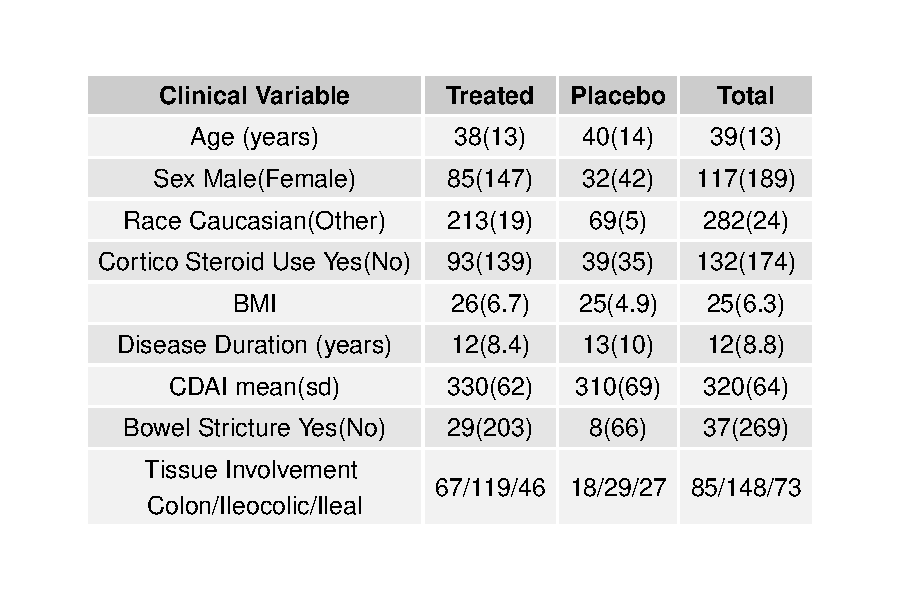
\includegraphics{tables/SupTable1_baseline_metadata.pdf}

\newpage

\textbf{Supplemental Table 1: Diversity differences based on clinical
metadata of chort at baseline}

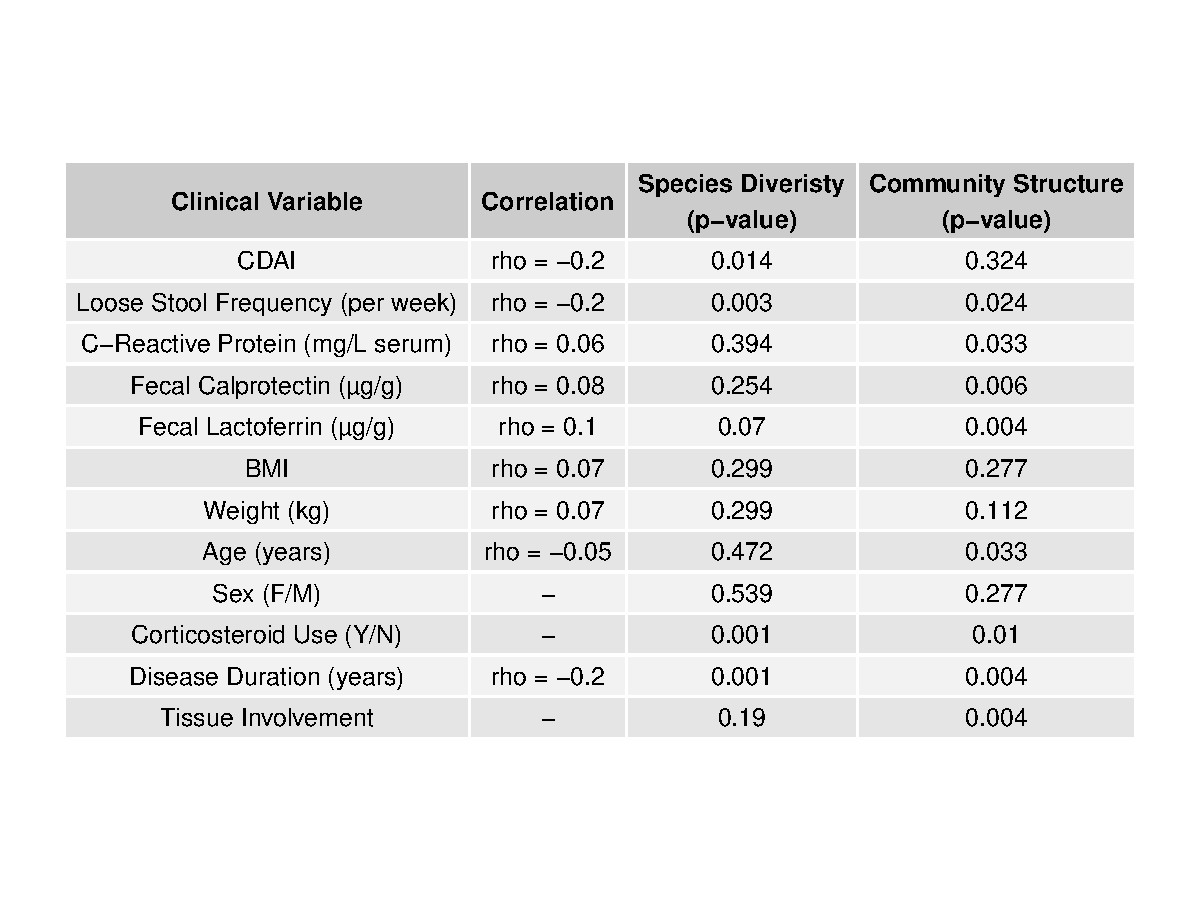
\includegraphics{tables/table1_cohortdiversity.pdf}

\newpage

\textbf{Table 2: Diversity differenced bases on Response/Remission in
UST treated subjects.}

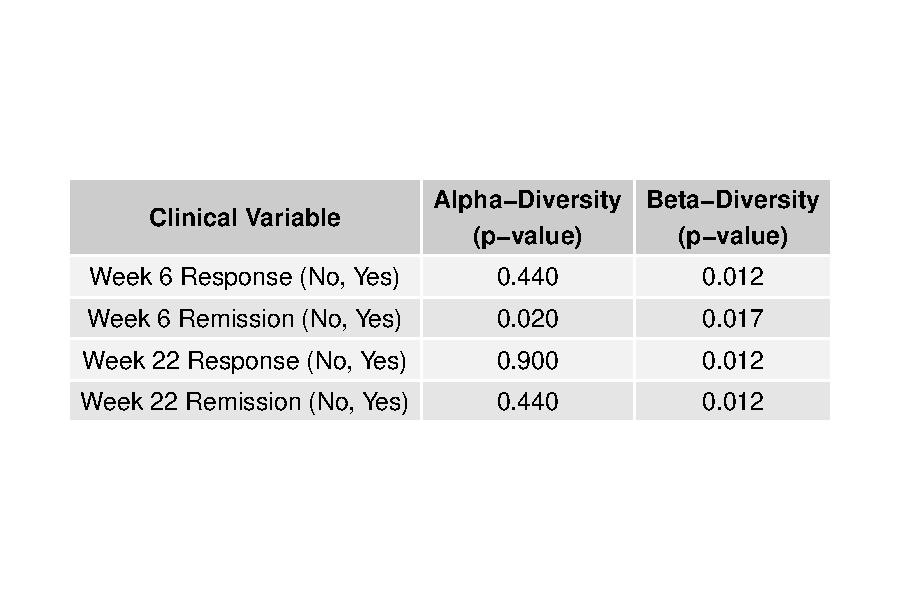
\includegraphics{tables/table2diversity.pdf}

\newpage

\subsection{Figures}\label{figures}

\textbf{Figure 1: Experimental design as adapted from Sanborne et al
2012.} (A) Diagram of experimetnal design and (B) stool sampling,
treatment, and response evalution timeline.

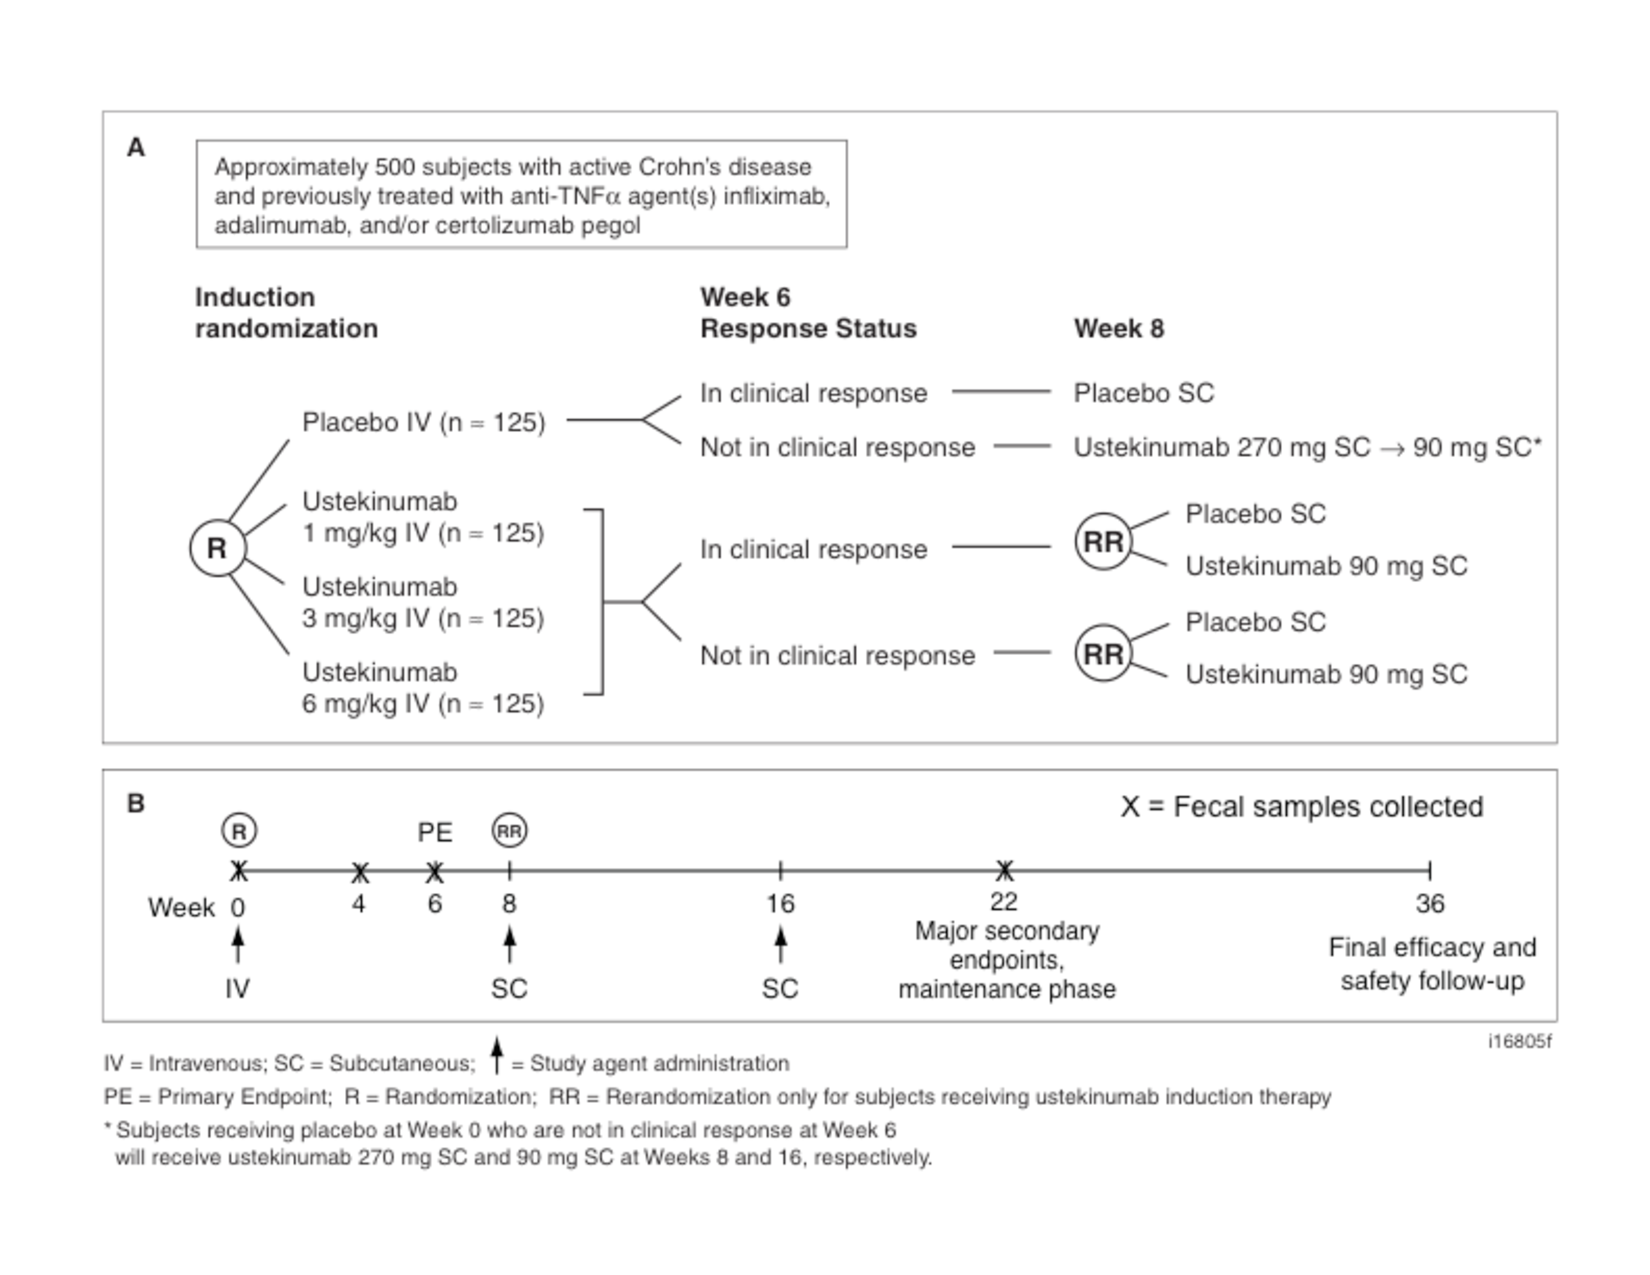
\includegraphics{figures/Figure1_expdesign.pdf}

\newpage

\textbf{Figure 2: Phyla from week 0 stool samples in subjects treated
with UST by week 6 outcome} (A) Response and (B) remission status.

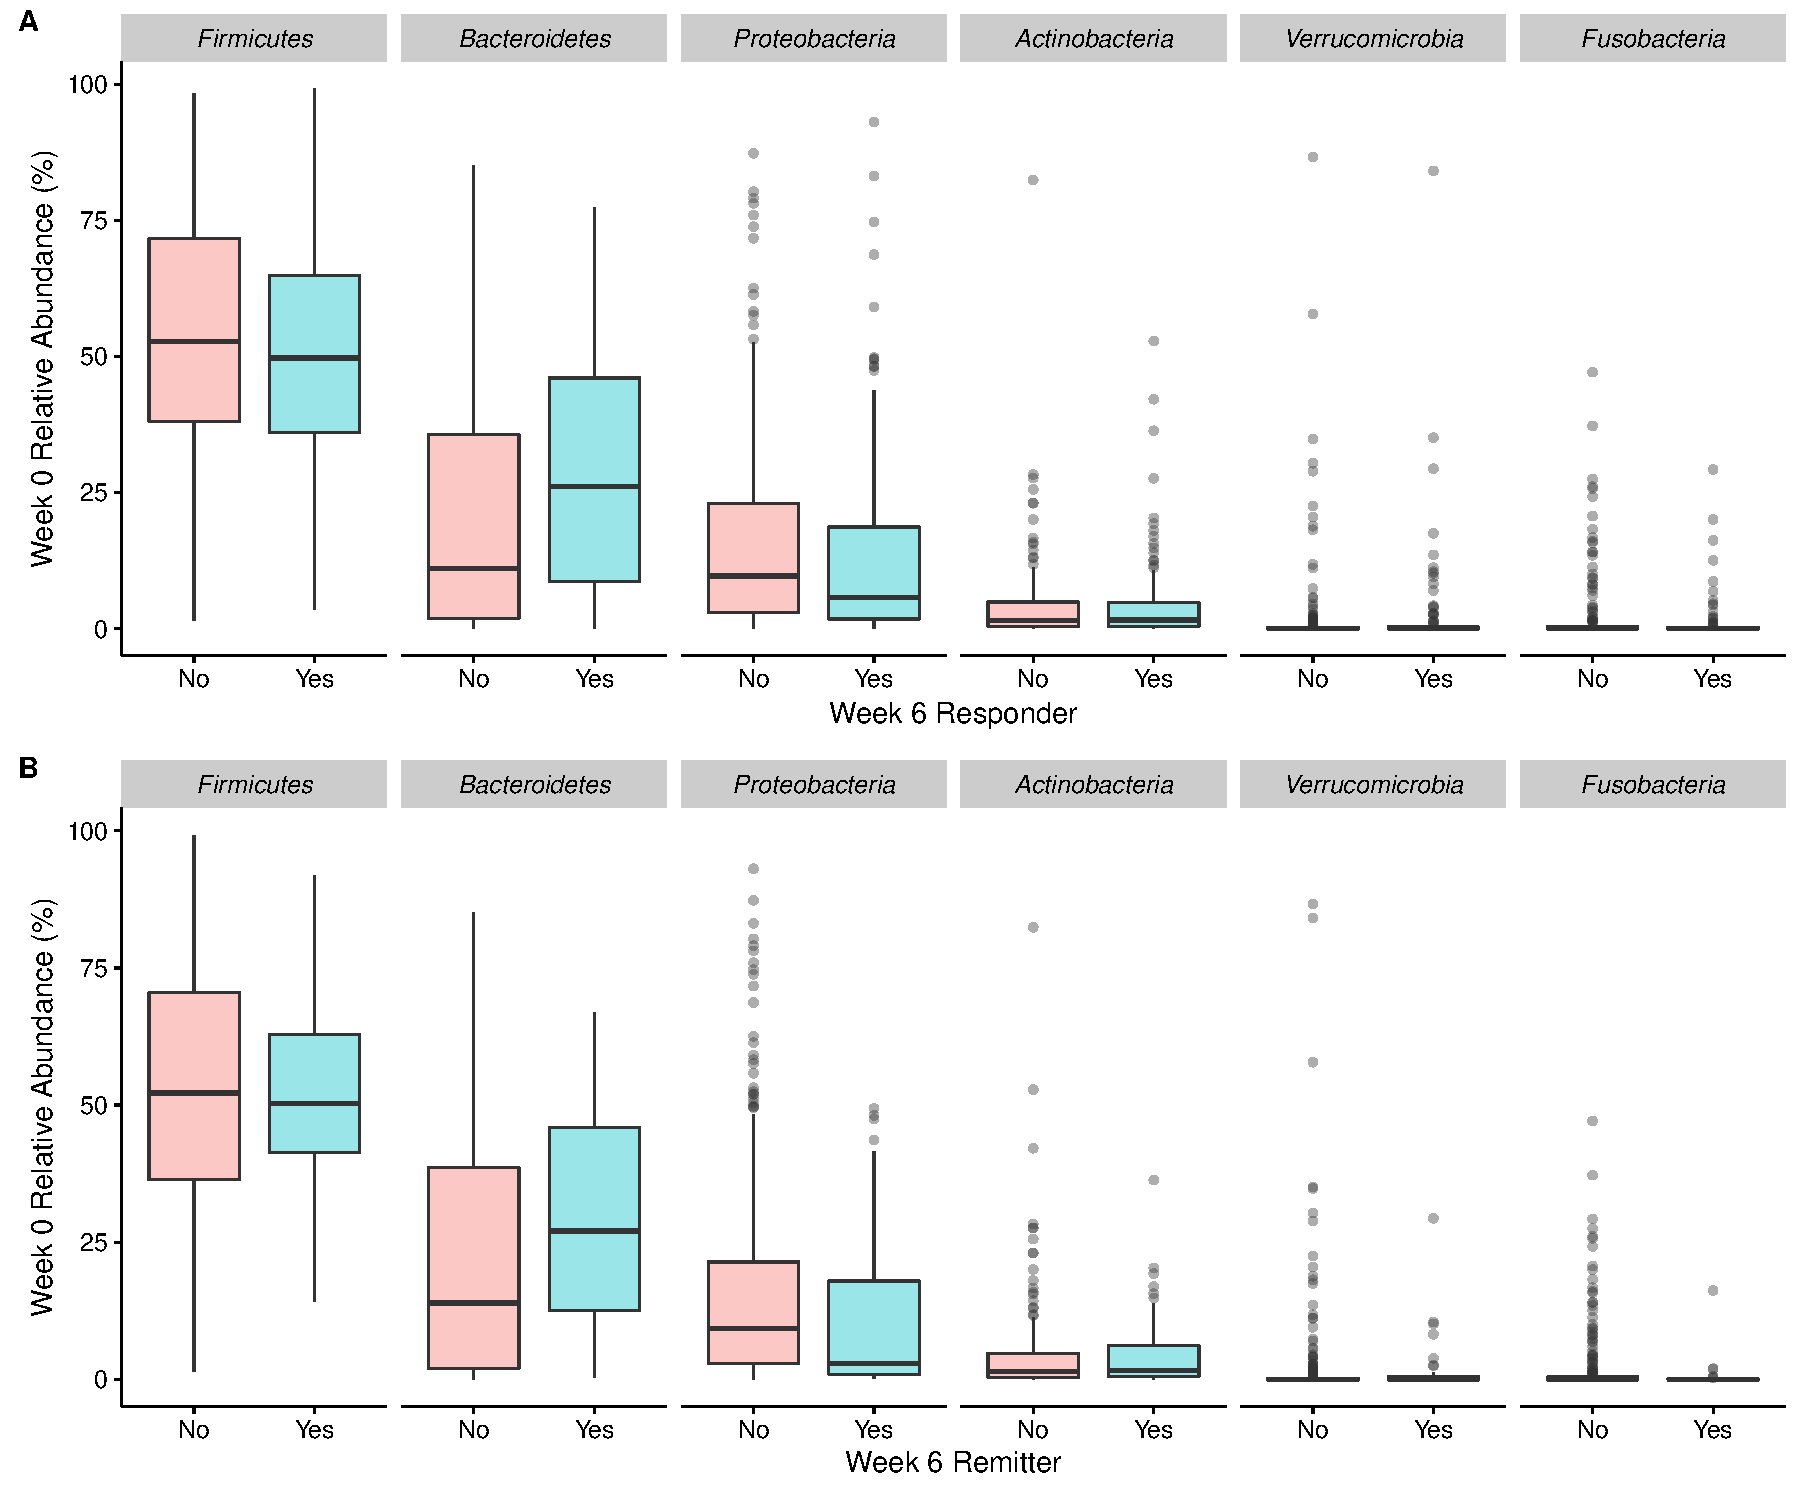
\includegraphics{figures/Figure2_wk6phyla.pdf}

\newpage

\textbf{Supplemental Figure 1: Phyla from week 0 stool samples in
subjects treated and maintained with UST by week 22 outcome} (A)
Response and (B) remission status.

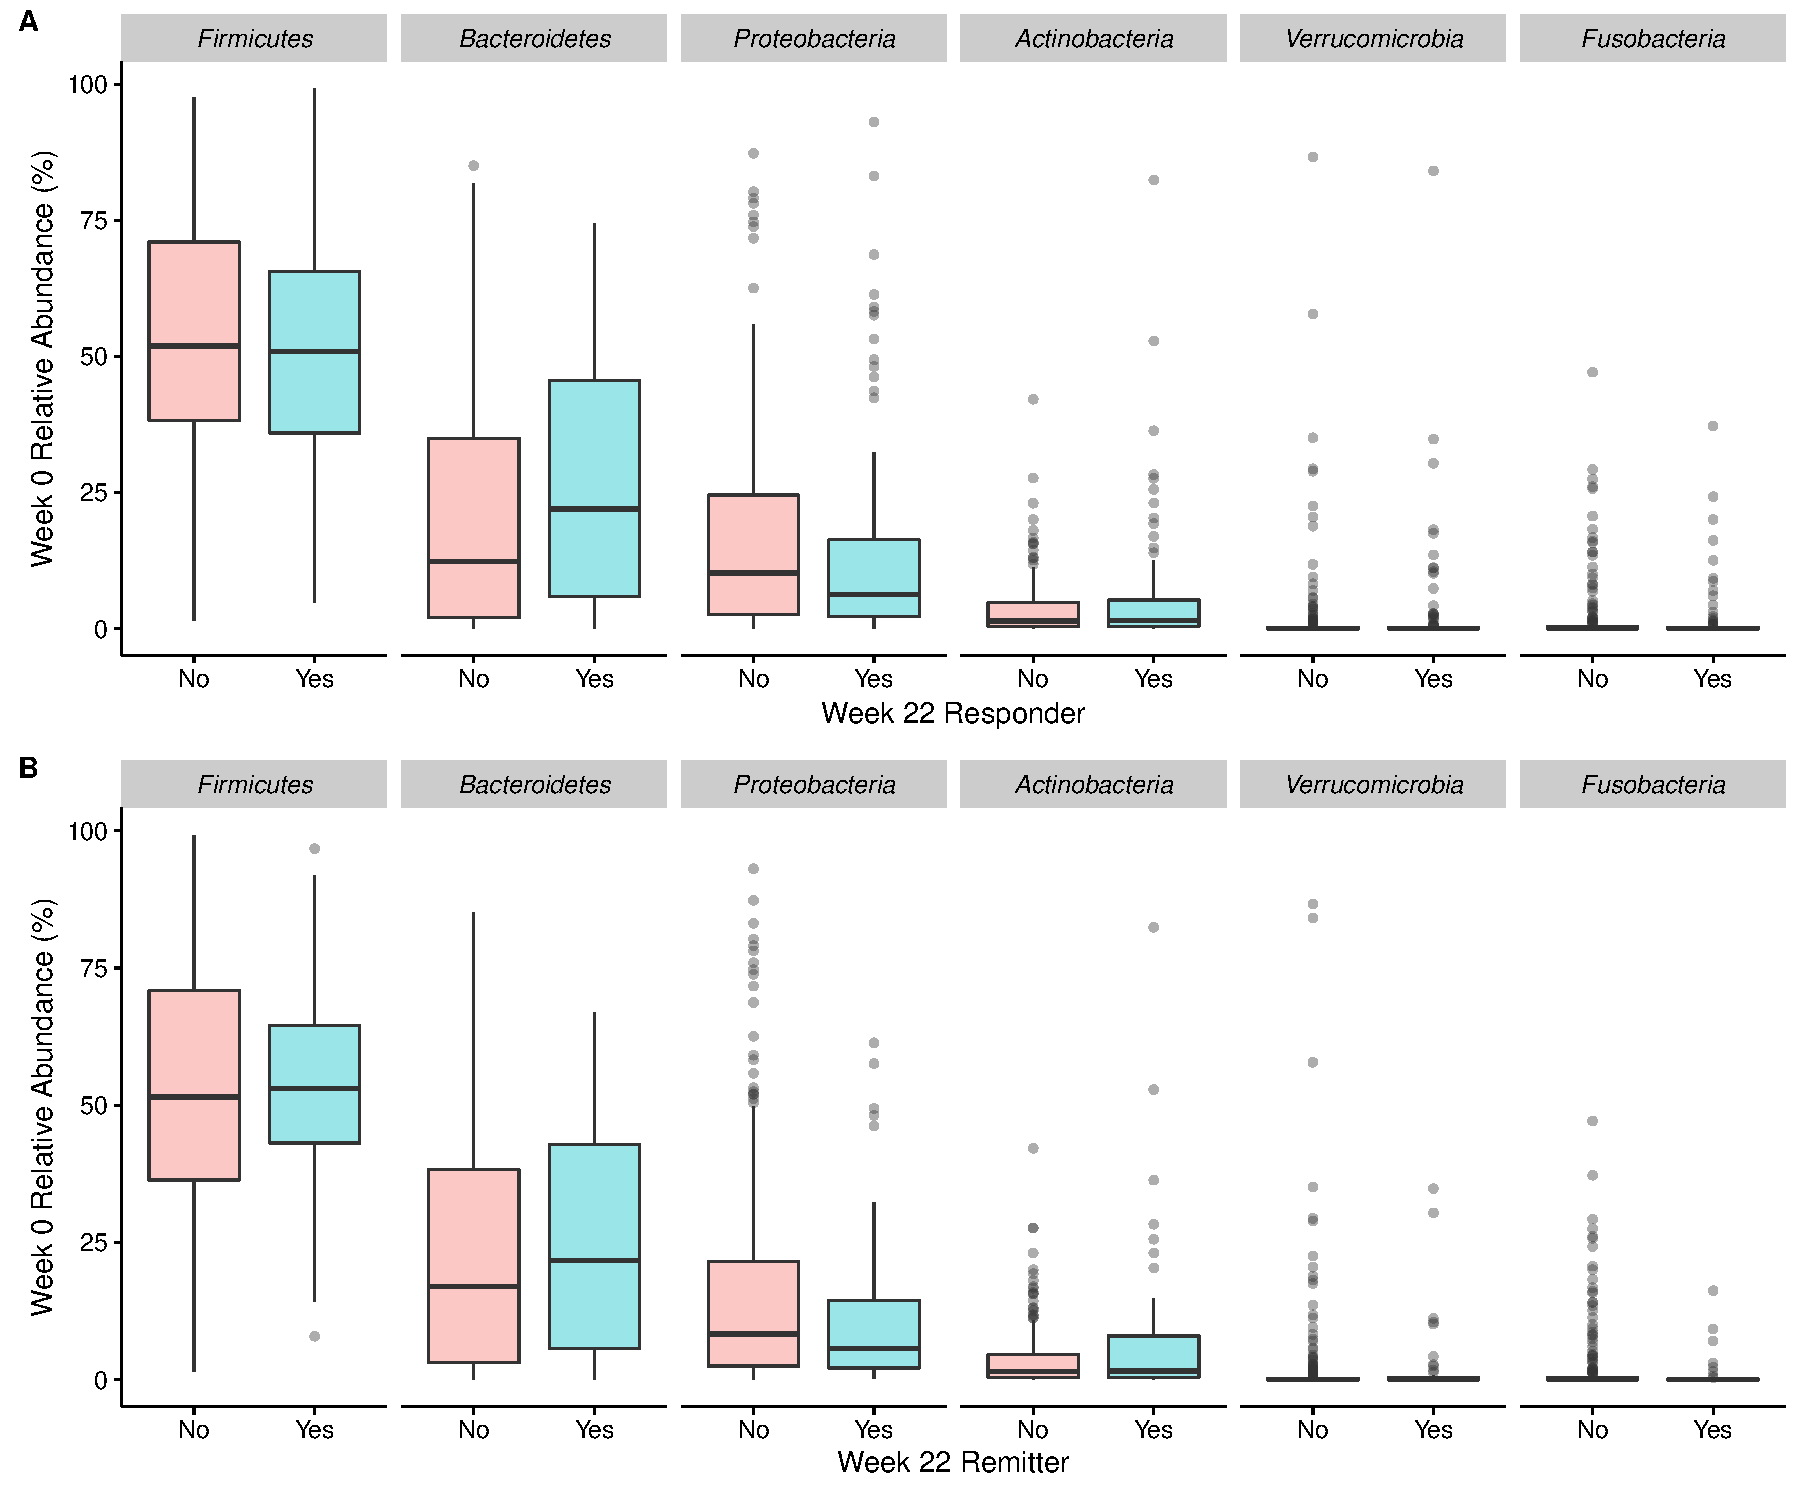
\includegraphics{figures/SF1_phylaWK22.pdf}

\newpage

\textbf{Figure 3: Differential taxa in week 0 stool samples from
subjects treated with UST, based on week 6 remission status}

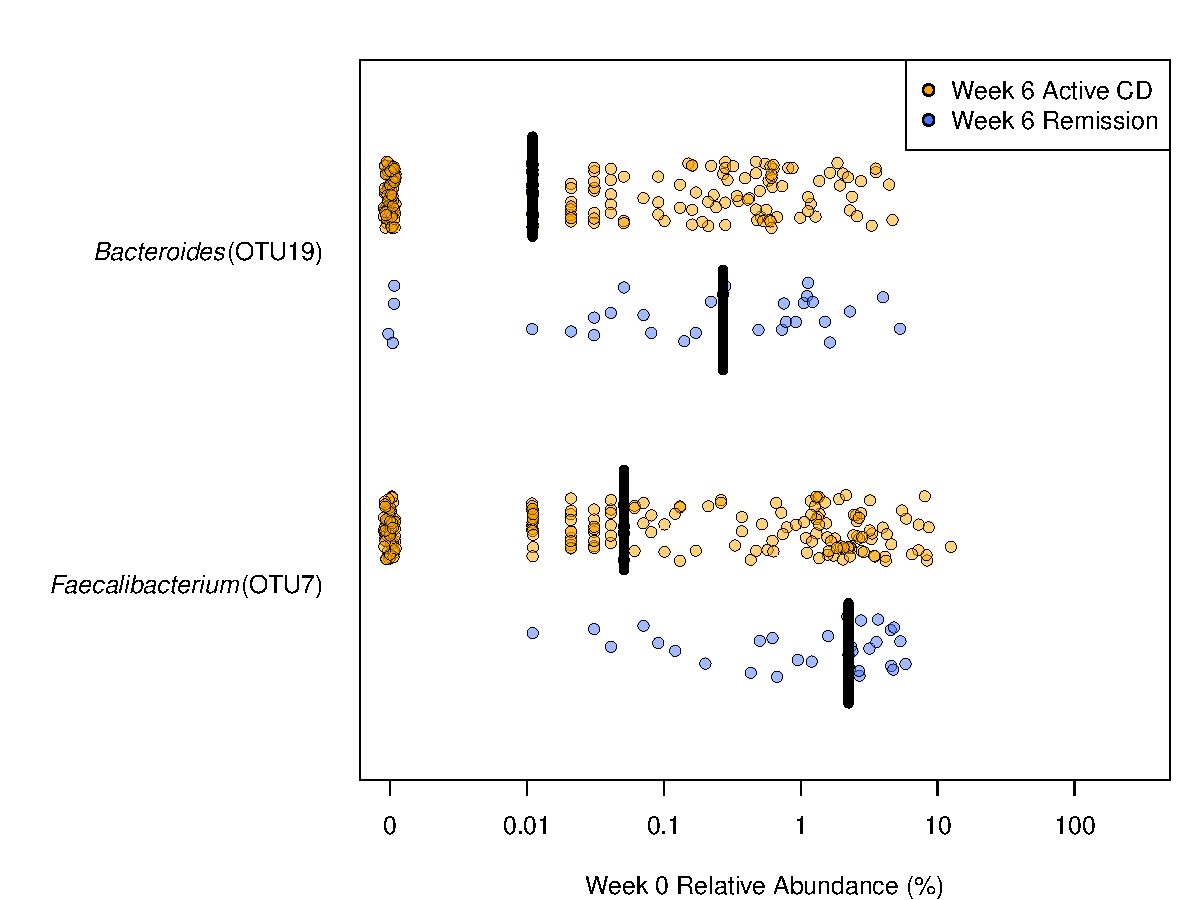
\includegraphics{figures/Figure3_basesigOTUabund.REMISSwk6.pdf}

\newpage

\textbf{Figure 4: Change in alpha diversity over time by induction
treatment and week 22 response status.}

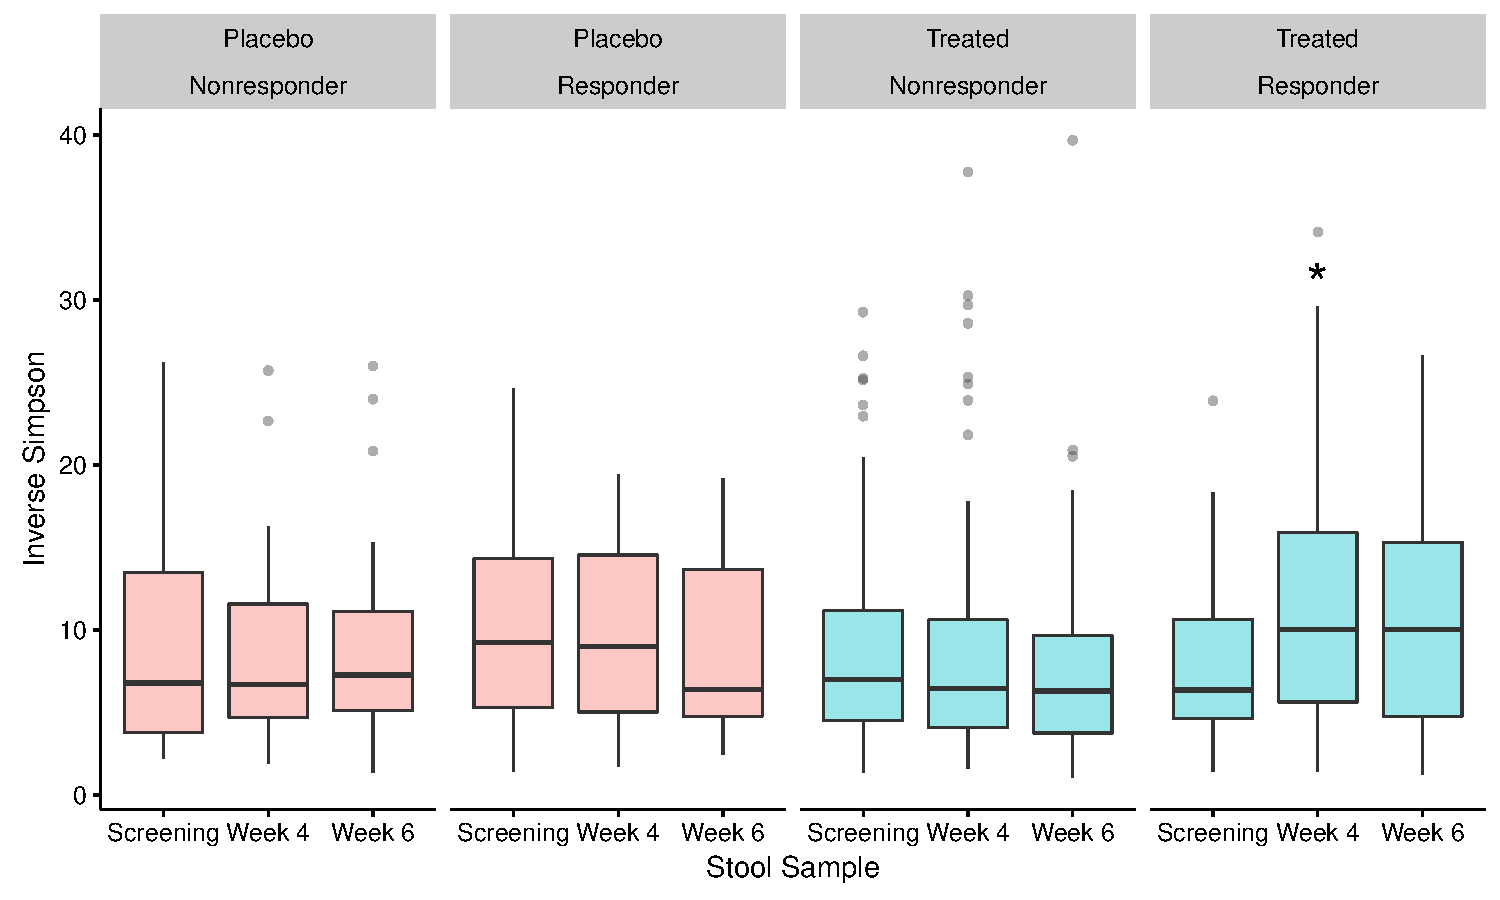
\includegraphics{figures/Figure4_wk046.adivXvisitXindtrtXrelRSPwk22.pdf}

\newpage

\textbf{Figure 5: Classification of week 6 response or remission status
using week 6 stool samples from subjects treated with UST} (A) ROCs for
week 6 outcome based on the microbiome. (B) Top predictive taxa from
week 6 stool for remission status at week 6.

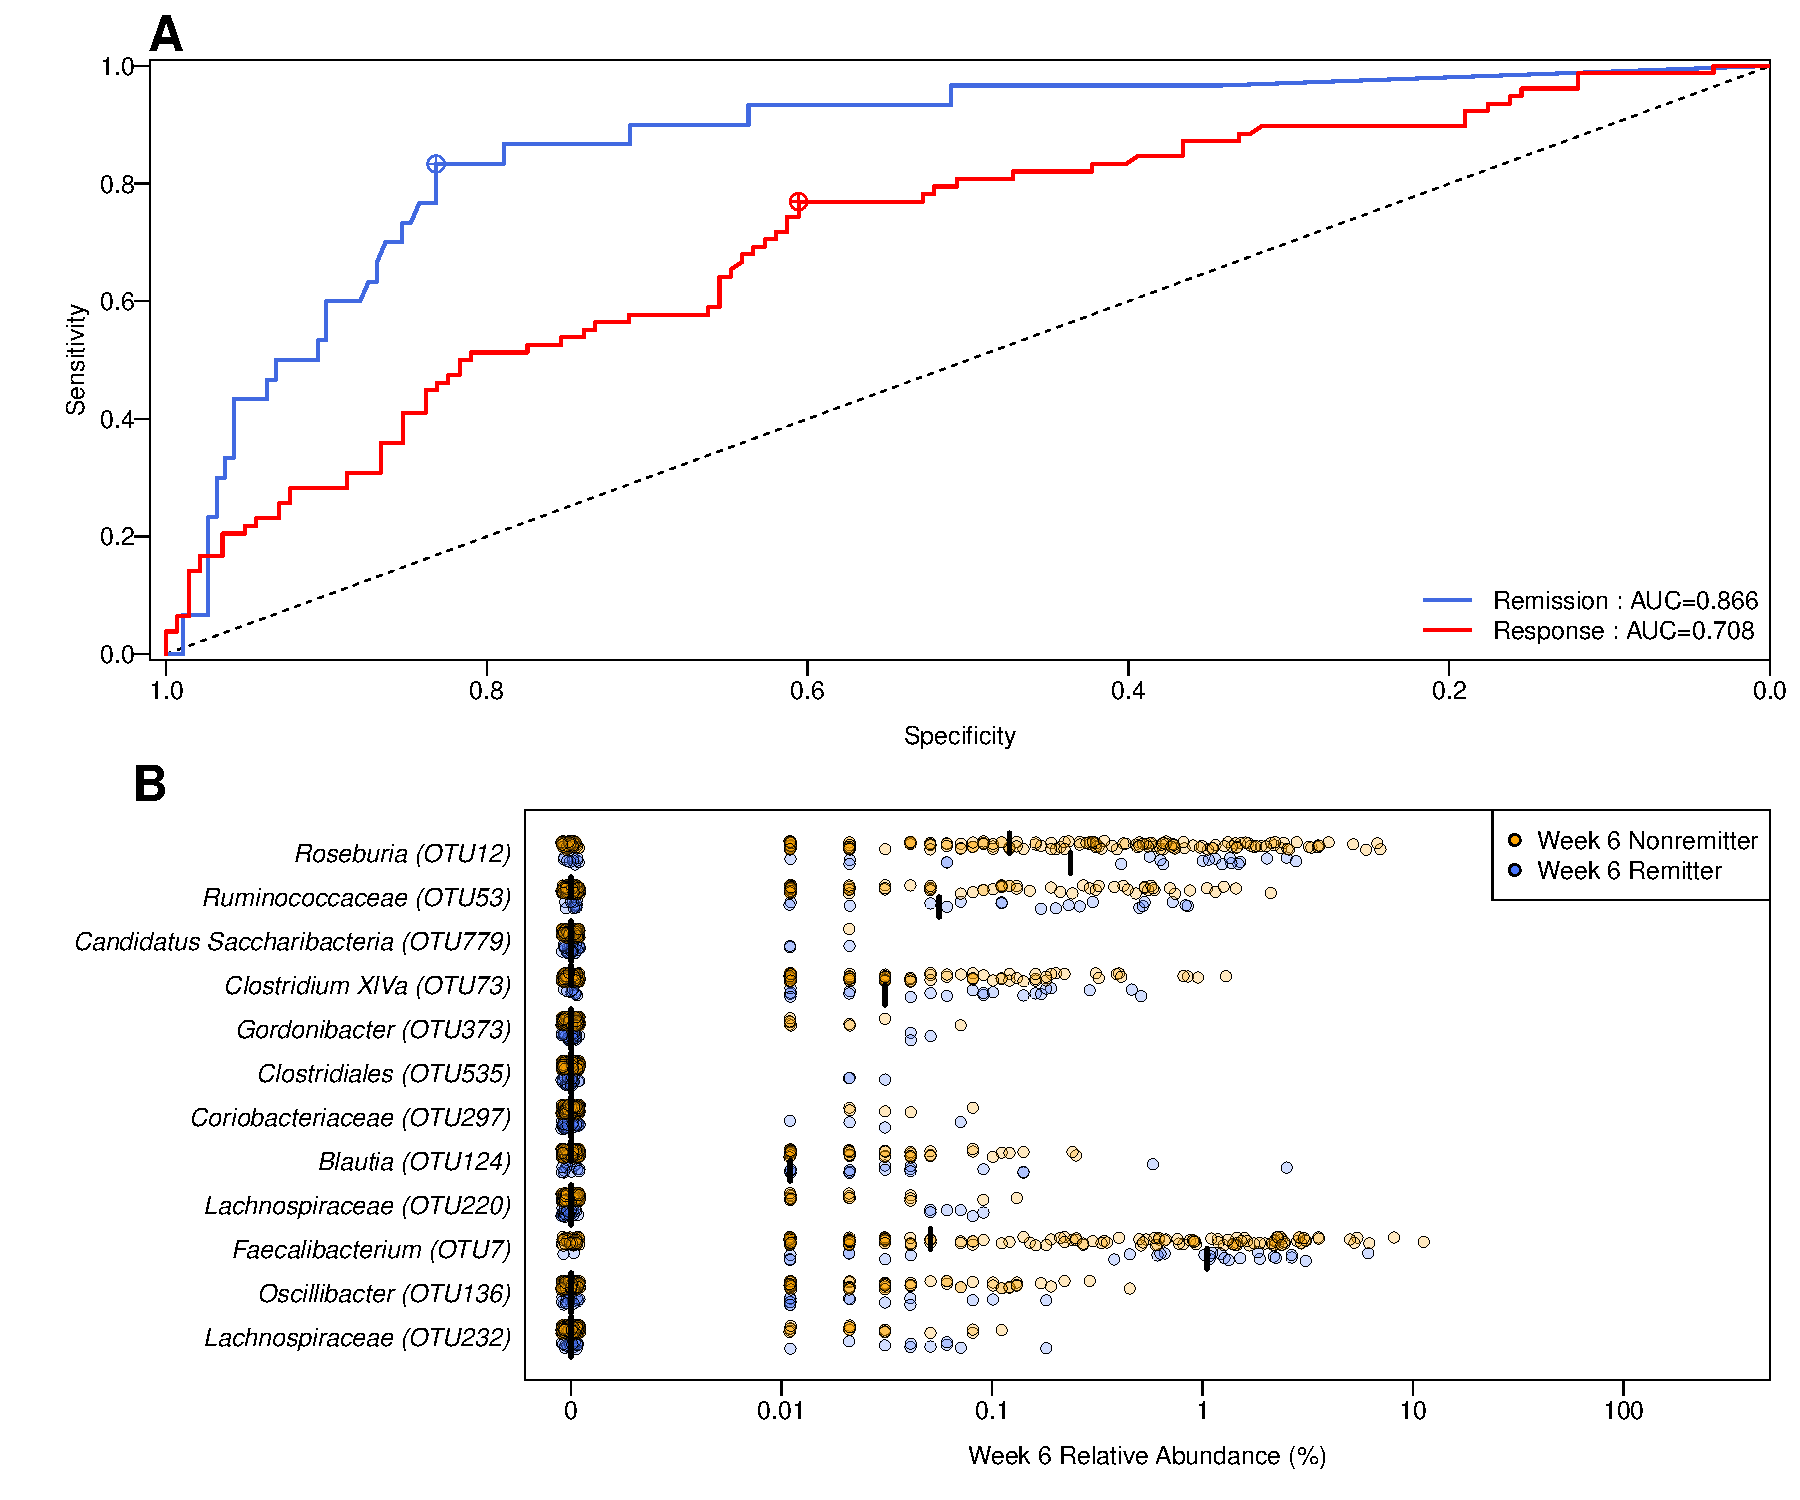
\includegraphics{figures/Figure5_wk6Xwk6.pdf}

\newpage

\textbf{Figure 6: Prediction of week 6 disease status in subjects
treated with UST, using week 0 samples} ROCs for (A) response and (C)
remission using microbiome data, clinical metadata, and the combined
model. Top predictive taxa for the microbiome model based on MDA for (B)
response and (D) remission.

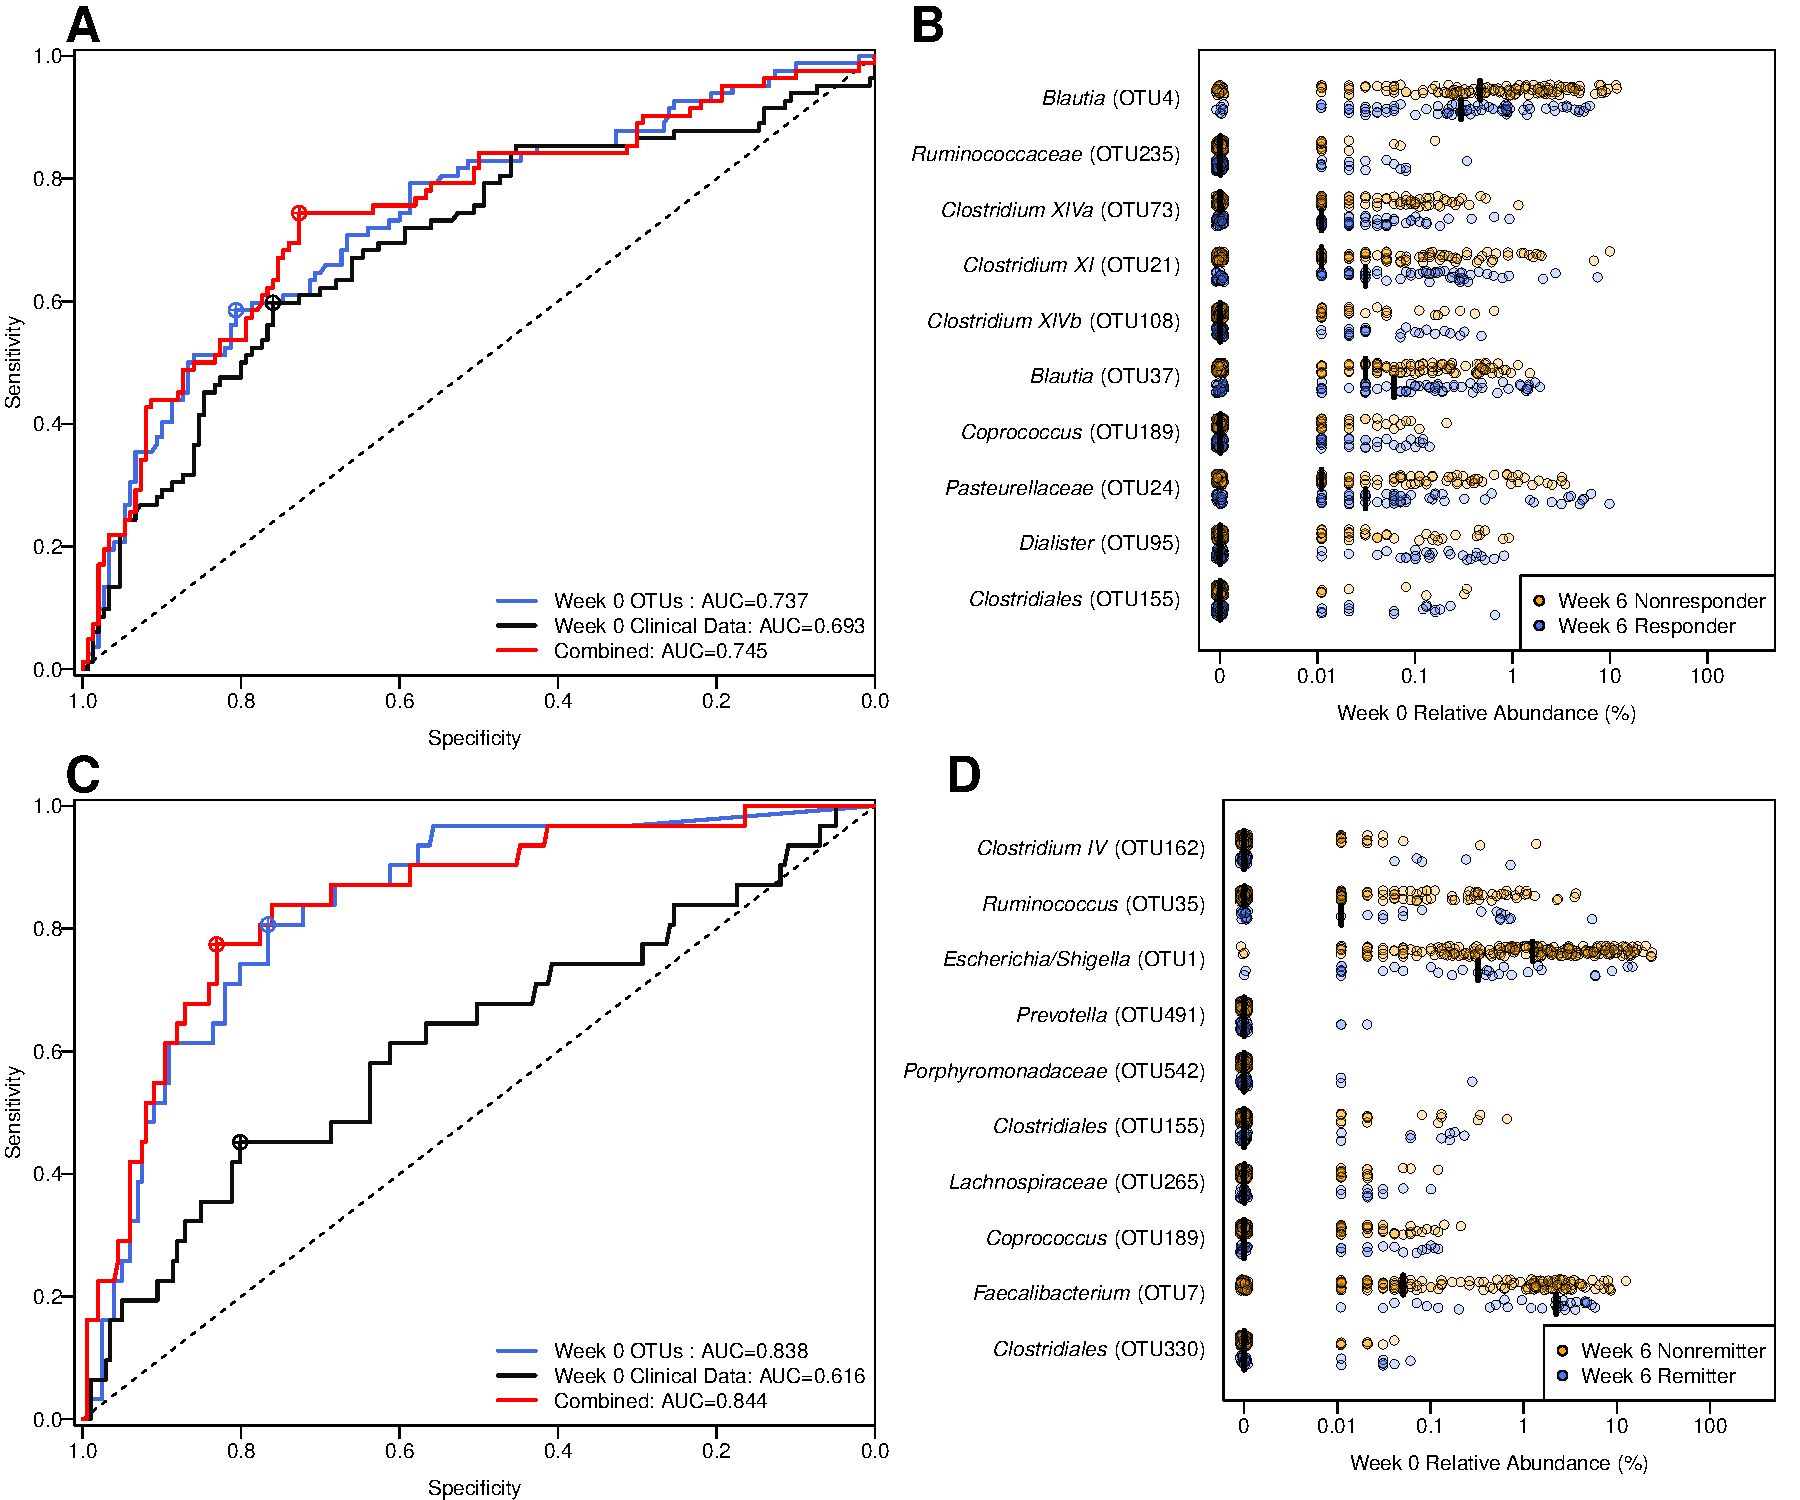
\includegraphics{figures/Figure6_wk0Xwk6pred.pdf}

\newpage

\textbf{Supplemental Figure 2: Predicting week 22 disease status in
subjects treated and maintained with UST, using week 0 samples} ROCs for
(A) response and (C) remission using microbiome data, clinical metadata,
and the combined model. Top predictive taxa for the microbiome model
based on MDA for (B) response and (D) remission.

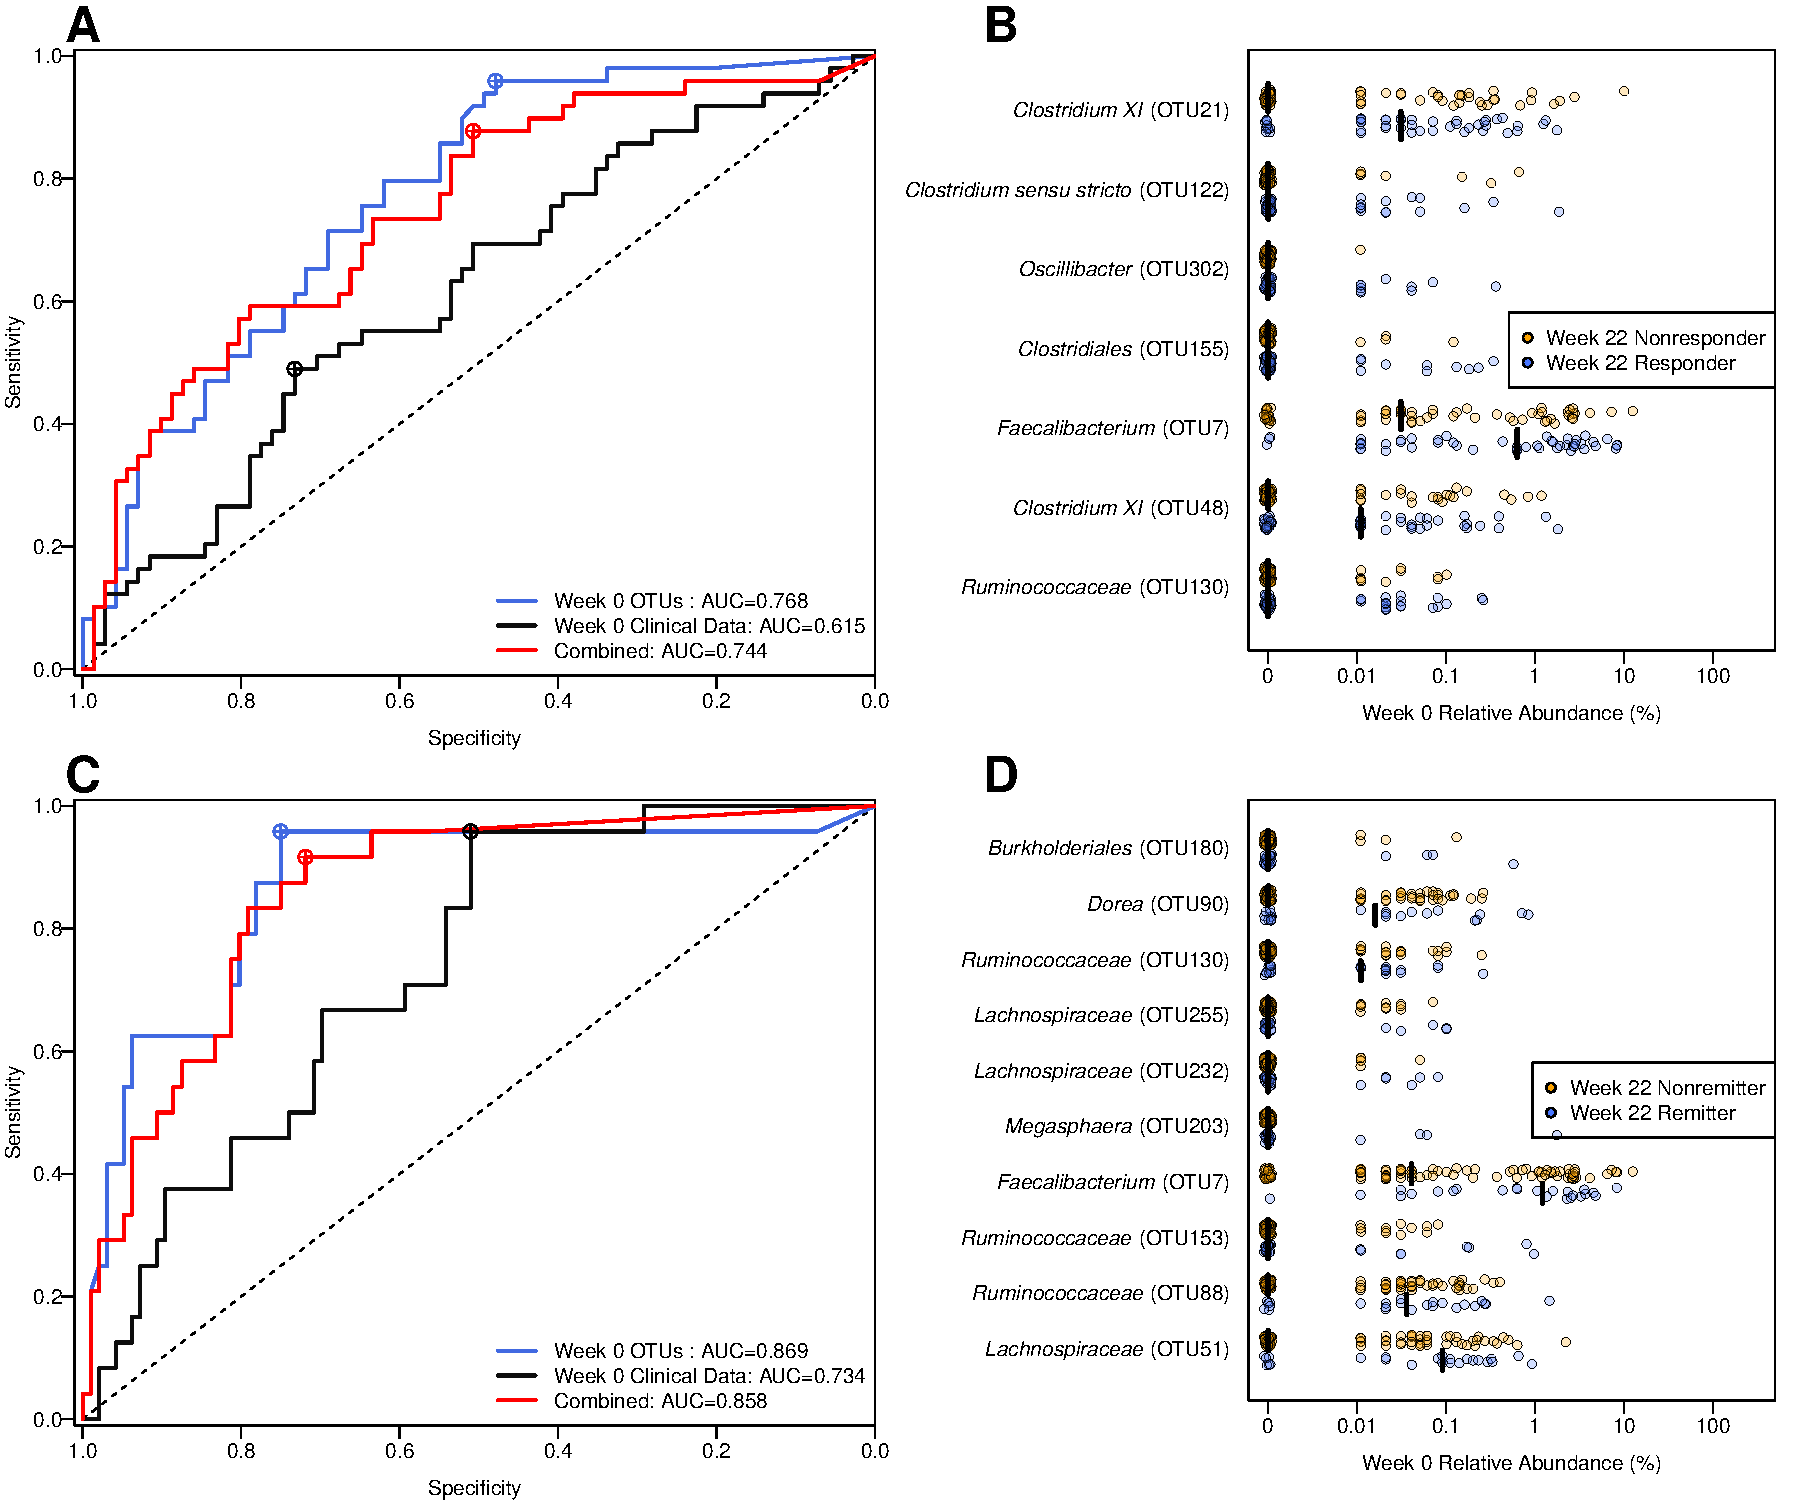
\includegraphics{figures/SF2-wk22predfig.pdf}

\newpage

\section*{References}\label{references}
\addcontentsline{toc}{section}{References}

\hypertarget{refs}{}
\hypertarget{ref-ananthakrishnan_epidemiology_2015}{}
1. Ananthakrishnan AN. 2015. Epidemiology and risk factors for IBD. Nat
Rev Gastroenterol Hepatol 12:205--217.

\hypertarget{ref-floyd_economicburden_2015}{}
2. Floyd DN, Langham S, Severac HC, Levesque BG. 2015. The economic and
quality-of-life burden of crohn's disease in europe and the united
states, 2000 to 2013: A systematic review. Dig Dis Sci 60:299--312.

\hypertarget{ref-molodecky_increasingIBD_2012}{}
3. Molodecky NA, Soon IS, Rabi DM, Ghali WA, Ferris M, Chernoff G,
Benchimol EI, Panaccione R, Ghosh S, Barkema HW, Kaplan GG. 2012.
Increasing incidence and prevalence of the inflammatory bowel diseases
with time, based on systematic review. Gastroenterology 142:46--54.e42;
quiz e30.

\hypertarget{ref-randall_CDbiologics_2015}{}
4. Randall CW, Vizuete JA, Martinez N, Alvarez JJ, Garapati KV,
Malakouti M, Taboada CM. 2015. From historical perspectives to modern
therapy: A review of current and future biological treatments for
crohn's disease. Therap Adv Gastroenterol 8:143--59.

\hypertarget{ref-wils_ust_2015}{}
5. Wils P, Bouhnik Y, Michetti P, Flourie B, Brixi H, Bourrier A, Allez
M, Duclos B, Grimaud JC, Buisson A, Amiot A, Fumery M, Roblin X,
Peyrin-Biroulet L, Filippi J, Bouguen G, Abitbol V, Coffin B, Simon M,
Laharie D, Pariente B. 2015. Subcutaneous ustekinumab provides clinical
benefit for two-thirds of patients with crohn's disease refractory to
anti-tumor necrosis factor agents. Clin Gastroenterol Hepatol.

\hypertarget{ref-colombel_deepremission_2015}{}
6. Colombel JF, Reinisch W, Mantzaris GJ, Kornbluth A, Rutgeerts P, Tang
KL, Oortwijn A, Bevelander GS, Cornillie FJ, Sandborn WJ. 2015.
Randomised clinical trial: Deep remission in biologic and
immunomodulator naive patients with crohn's disease - a SONIC post hoc
analysis. Aliment Pharmacol Ther 41:734--46.

\hypertarget{ref-baert_mucosalhealing_2010}{}
7. Baert F, Moortgat L, Van Assche G, Caenepeel P, Vergauwe P, De Vos M,
Stokkers P, Hommes D, Rutgeerts P, Vermeire S, D'Haens G. 2010. Mucosal
healing predicts sustained clinical remission in patients with
early-stage crohn's disease. Gastroenterology 138:463--8; quiz e10--1.

\hypertarget{ref-sartor_IBDpath_2006}{}
8. Sartor RB. 2006. Mechanisms of disease: Pathogenesis of crohn's
disease and ulcerative colitis. Nat Clin Pract Gastroenterol Hepatol
3:390--407.

\hypertarget{ref-wright_CDmicrobiome_2015}{}
9. Wright EK, Kamm MA, Teo SM, Inouye M, Wagner J, Kirkwood CD. 2015.
Recent advances in characterizing the gastrointestinal microbiome in
crohn's disease: A systematic review. Inflamm Bowel Dis 21:1219--28.

\hypertarget{ref-manichanh_diversityCD_2006}{}
10. Manichanh C, Rigottier-Gois L, Bonnaud E, Gloux K, Pelletier E,
Frangeul L, Nalin R, Jarrin C, Chardon P, Marteau P, Roca J, Dore J.
2006. Reduced diversity of faecal microbiota in crohn's disease revealed
by a metagenomic approach. Gut 55:205--11.

\hypertarget{ref-hansen_pedsIBD_2012}{}
11. Hansen R, Russell RK, Reiff C, Louis P, McIntosh F, Berry SH,
Mukhopadhya I, Bisset WM, Barclay AR, Bishop J, Flynn DM, McGrogan P,
Loganathan S, Mahdi G, Flint HJ, El-Omar EM, Hold GL. 2012. Microbiota
of de-novo pediatric IBD: Increased faecalibacterium prausnitzii and
reduced bacterial diversity in crohn's but not in ulcerative colitis. Am
J Gastroenterol 107:1913--22.

\hypertarget{ref-haberman_pedsCD_2014}{}
12. Haberman Y, Tickle TL, Dexheimer PJ, Kim MO, Tang D, Karns R,
Baldassano RN, Noe JD, Rosh J, Markowitz J, Heyman MB, Griffiths AM,
Crandall WV, Mack DR, Baker SS, Huttenhower C, Keljo DJ, Hyams JS,
Kugathasan S, Walters TD, Aronow B, Xavier RJ, Gevers D, Denson LA.
2014. Pediatric crohn disease patients exhibit specific ileal
transcriptome and microbiome signature. J Clin Invest 124:3617--33.

\hypertarget{ref-gevers_pedsCD_2014}{}
13. Gevers D, Kugathasan S, Denson LA, Vazquez-Baeza Y, Van Treuren W,
Ren B, Schwager E, Knights D, Song SJ, Yassour M, Morgan XC, Kostic AD,
Luo C, Gonzalez A, McDonald D, Haberman Y, Walters T, Baker S, Rosh J,
Stephens M, Heyman M, Markowitz J, Baldassano R, Griffiths A, Sylvester
F, Mack D, Kim S, Crandall W, Hyams J, Huttenhower C, Knight R, Xavier
RJ. 2014. The treatment-naive microbiome in new-onset crohn's disease.
Cell Host Microbe 15:382--92.

\hypertarget{ref-Huang_gingivitis_2014}{}
14. Huang S, Li R, Zeng X, He T, Zhao H, Chang A, Bo C, Chen J, Yang F,
Knight R, Liu J, Davis C, Xu J. 2014. Predictive modeling of gingivitis
severity and susceptibility via oral microbiota. ISME J 8:1768--80.

\hypertarget{ref-Wang_cvdrisk_2016}{}
15. Wang Y, Ames NP, Tun HM, Tosh SM, Jones PJ, Khafipour E. 2016. High
molecular weight barley β-glucan alters gut microbiota toward reduced
cardiovascular disease risk. Front Microbiol 7.

\hypertarget{ref-Schubert_cdiff_2016}{}
16. Schubert AM, Sinani H, Schloss PD. 2015. Antibiotic-induced
alterations of the murine gut microbiota and subsequent effects on
colonization resistance against clostridium difficile. MBio 6:e00974.

\hypertarget{ref-Schubert_cdiff_2014}{}
17. Schubert AM, Rogers MAM, Ring C, Mogle J, Petrosino JP, Young VB,
Aronoff DM, Schloss PD. 2014. Microbiome data distinguish patients with
clostridium difficile infection and non-c. difficile-associated diarrhea
from healthy controls. mBio 5.

\hypertarget{ref-Seekatz_cdiff_2016}{}
18. Seekatz AM, Rao K, Santhosh K, Young VB. 2016. Dynamics of the fecal
microbiome in patients with recurrent and nonrecurrent clostridium
difficile infection. Genome Med 8.

\hypertarget{ref-zackular_CRC_2014}{}
19. Zackular JP, Rogers MA, Ruffin MT th, Schloss PD. 2014. The human
gut microbiome as a screening tool for colorectal cancer. Cancer Prev
Res (Phila) 7:1112--21.

\hypertarget{ref-baxter_FIT_2016}{}
20. Baxter NT, Ruffin MT th, Rogers MA, Schloss PD. 2016.
Microbiota-based model improves the sensitivity of fecal immunochemical
test for detecting colonic lesions. Genome Med 8:37.

\hypertarget{ref-wang_pedsCD_2016}{}
21. Wang F, Kaplan JL, Gold BD, Bhasin MK, Ward NL, Kellermayer R,
Kirschner BS, Heyman MB, Dowd SE, Cox SB, Dogan H, Steven B, Ferry GD,
Cohen SA, Baldassano RN, Moran CJ, Garnett EA, Drake L, Otu HH, Mirny
LA, Libermann TA, Winter HS, Korolev KS. 2016. Detecting microbial
dysbiosis associated with pediatric crohn disease despite the high
variability of the gut microbiota. Cell Rep.

\hypertarget{ref-Ananthakrishnan_IBD_2017}{}
22. Ananthakrishnan AN, Luo C, Yajnik V, Khalili H, Garber JJ, Stevens
BW, Cleland T, Xavier RJ. 2017. Gut microbiome function predicts
response to anti-integrin biologic therapy in inflammatory bowel
diseases. Cell Host Microbe 21:603--610.e3.

\hypertarget{ref-sandborn_ust_2012}{}
23. Sandborn WJ, Gasink C, Gao LL, Blank MA, Johanns J, Guzzo C, Sands
BE, Hanauer SB, Targan S, Rutgeerts P, Ghosh S, Villiers WJ de,
Panaccione R, Greenberg G, Schreiber S, Lichtiger S, Feagan BG. 2012.
Ustekinumab induction and maintenance therapy in refractory crohn's
disease. N Engl J Med 367:1519--28.

\hypertarget{ref-sandborn_ust_2008}{}
24. Sandborn WJ, Feagan BG, Fedorak RN, Scherl E, Fleisher MR, Katz S,
Johanns J, Blank M, Rutgeerts P. 2008. A randomized trial of
ustekinumab, a human interleukin-12/23 monoclonal antibody, in patients
with moderate-to-severe crohn's disease. Gastroenterology 135:1130--41.

\hypertarget{ref-kopylov_ust_2014}{}
25. Kopylov U, Afif W, Cohen A, Bitton A, Wild G, Bessissow T, Wyse J,
Al-Taweel T, Szilagyi A, Seidman E. 2014. Subcutaneous ustekinumab for
the treatment of anti-TNF resistant crohn's disease--the McGill
experience. J Crohns Colitis 8:1516--22.

\hypertarget{ref-schloss_mothur_2009}{}
26. Schloss PD, Westcott SL, Ryabin T, Hall JR, Hartmann M, Hollister
EB, Lesniewski RA, Oakley BB, Parks DH, Robinson CJ, Sahl JW, Stres B,
Thallinger GG, Van Horn DJ, Weber CF. 2009. Introducing mothur:
Open-source, platform-independent, community-supported software for
describing and comparing microbial communities. Appl Environ Microbiol
75:7537--41.

\hypertarget{ref-oksanen_vegan_2016}{}
27. Oksanen J, Blanchet FG, Friendly M, Kindt R, Legendre P, McGlinn D,
Minchin PR, O'Hara RB, Simpson GL, Solymos P, Stevens MHH, Szoecs E,
Wagner H. 2016. Vegan: Community ecology package. r package version
2.4-1.

\hypertarget{ref-tedjo_CDactivity_2016}{}
28. Tedjo DI, Smolinska A, Savelkoul PH, Masclee AA, Schooten FJ van,
Pierik MJ, Penders J, Jonkers DMAE. 2016. The fecal microbiota as a
biomarker for disease activity in crohn's disease. Scientific Reports,
Published online: 13 October 2016; doi:101038/srep35216.

\hypertarget{ref-calle_aucrf_2011}{}
29. Calle ML, Urrea V, Boulesteix A-L, Malats N. 2011. AUC-RF: A new
strategy for genomic profiling with random forest. Human Heredity
72:121--132.

\hypertarget{ref-boon_fmarkers_2015}{}
30. Boon GJ, Day AS, Mulder CJ, Gearry RB. 2015. Are faecal markers good
indicators of mucosal healing in inflammatory bowel disease? World J
Gastroenterol 21:11469--80.

\hypertarget{ref-chang_monitoring_2015}{}
31. Chang S, Malter L, Hudesman D. 2015. Disease monitoring in
inflammatory bowel disease. World J Gastroenterol 21:11246--59.

\hypertarget{ref-papa_pedsIBD_2012}{}
32. Papa E, Docktor M, Smillie C, Weber S, Preheim SP, Gevers D,
Giannoukos G, Ciulla D, Tabbaa D, Ingram J, Schauer DB, Ward DV,
Korzenik JR, Xavier RJ, Bousvaros A, Alm EJ. 2012. Non-invasive mapping
of the gastrointestinal microbiota identifies children with inflammatory
bowel disease. PLoS One 7:e39242.

\hypertarget{ref-vandeputte_stoolcon_2016}{}
33. Vandeputte D, Falony G, Vieira-Silva S, Tito RY, Joossens M, Raes J.
2016. Original article: Stool consistency is strongly associated with
gut microbiota richness and composition, enterotypes and bacterial
growth rates. Gut 65:57--62.

\hypertarget{ref-naftali_tissinvol_2016}{}
34. Naftali T, Reshef L, Kovacs A, Porat R, Amir I, Konikoff FM, Gophna
U. 2016. Distinct microbiotas are associated with ileum-restricted and
colon-involving crohn's disease. Inflamm Bowel Dis 22:293--302.

\hypertarget{ref-huang_cort_2015}{}
35. Huang EY, Inoue T, Leone VA, Dalal S, Touw K, Wang Y, Musch MW,
Theriault B, Higuchi K, Donovan S, Gilbert J, Chang EB. 2015. Using
corticosteroids to reshape the gut microbiome: Implications for
inflammatory bowel diseases. Inflamm Bowel Dis 21:963--72.

\hypertarget{ref-monteleone_mongersen_2015}{}
36. Monteleone G, Neurath MF, Ardizzone S, Di Sabatino A, Fantini MC,
Castiglione F, Scribano ML, Armuzzi A, Caprioli F, Sturniolo GC, Rogai
F, Vecchi M, Atreya R, Bossa F, Onali S, Fichera M, Corazza GR, Biancone
L, Savarino V, Pica R, Orlando A, Pallone F. 2015. Mongersen, an oral
SMAD7 antisense oligonucleotide, and crohn's disease. N Engl J Med
372:1104--13.

\hypertarget{ref-monteleone_mongersen_2016}{}
37. Monteleone G, Di Sabatino A, Ardizzone S, Pallone F, Usiskin K, Zhan
X, Rossiter G, Neurath MF. 2016. Impact of patient characteristics on
the clinical efficacy of mongersen (GED-0301), an oral smad7 antisense
oligonucleotide, in active crohn's disease. Aliment Pharmacol Ther
43:717--24.

\hypertarget{ref-ardizzone_mongersen_2016}{}
38. Ardizzone S, Bevivino G, Monteleone G. 2016. Mongersen, an oral
smad7 antisense oligonucleotide, in patients with active crohn's
disease. Therap Adv Gastroenterol 9:527--32.

\hypertarget{ref-orava_short_2013}{}
39. Orava EW, Jarvik N, Shek YL, Sidhu SS, Gariepy J. 2013. A short DNA
aptamer that recognizes TNFalpha and blocks its activity in vitro. ACS
Chem Biol 8:170--8.

\hypertarget{ref-sartor_microbesIBD_2016}{}
40. Sartor RB, Wu GD. 2016. Roles for intestinal bacteria, viruses, and
fungi in pathogenesis of inflammatory bowel diseases and therapeutic
approaches. Gastroenterology.

\hypertarget{ref-schloss_PCRartifacts_2011}{}
41. Schloss PD, Gevers D, Westcott SL. 2011. Reducing the effects of PCR
amplification and sequencing artifacts on 16S rRNA-based studies. PLoS
One 6:e27310.

\hypertarget{ref-edgar_uchime_2011}{}
42. Edgar RC, Haas BJ, Clemente JC, Quince C, Knight R. 2011. UCHIME
improves sensitivity and speed of chimera detection. Bioinformatics
27:2194--200.

\hypertarget{ref-schloss_OTUanalysis_2011}{}
43. Schloss PD, Westcott SL. 2011. Assessing and improving methods used
in operational taxonomic unit-based approaches for 16S rRNA gene
sequence analysis. Appl Environ Microbiol 77:3219--26.

\hypertarget{ref-wang_taxonomy_2007}{}
44. Wang Q, Garrity GM, Tiedje JM, Cole JR. 2007. Naive bayesian
classifier for rapid assignment of rRNA sequences into the new bacterial
taxonomy. Appl Environ Microbiol 73:5261--7.

\hypertarget{ref-sokal_biometrystats_1995}{}
45. Sokal RR, Rohlf FJ. 1995. Biometry: The principles and practice of
statistics in biological research, 3rd ed. Freeman, New York.

\hypertarget{ref-magurran_measuring_2004}{}
46. Magurran AE. 2004. Measuring biological diversity. Blackwell Pub.,
Malden, Ma.

\hypertarget{ref-yue_thetaYC_2005}{}
47. Yue JC, Clayton MK. 2005. A similarity measure based on species
proportions. Communications in Statistics-Theory and Methods
34:2123--2131.

\hypertarget{ref-schloss_commstruct_2008}{}
48. Schloss PD. 2008. Evaluating different approaches that test whether
microbial communities have the same structure. ISME J 2:265--75.

\hypertarget{ref-friedman_1937}{}
49. Friedman M. 1937. The use of ranks to avoid the assumption of
normality implicit in the analysis of variance. Journal of the American
Statistical Association 32:675--701.

\hypertarget{ref-Benjamini_Hochberg_1995}{}
50. Benjamini Y, Hochberg Y. 1995. Controlling the false discovery rate:
A practical and powerful approach to multiple testing. Journal of the
Royal Statistical Society Series B (Methodological) 57:289--300.

\hypertarget{ref-breiman_rf_2001}{}
51. Breiman L. 2001. Random forests. Machine Learning 45:5--32.


\end{document}
